

\chapter{大脑皮层平滑跟踪通路解剖对齐的视觉跟踪模型}
\label{chap:btn}
% 更接近于人 vs 更接近于神
% regressor  回归变量
% STS: superior temporal sulcus (STS)
% SEF: supplementary eye field (SEF)

\section{引言}
% BTN第一章第一段
作为多目标跟踪的基础,基于深度神经网络的单目标跟踪模型已经取得了巨大的进步~\cite{ILSVRC15},然而随之而来的是越来越复杂的模型和可解释性的缺失,导致单目标跟踪算法难以扩展到多目标场景,并严重制约了模型的理解与实际应用。
尽管更深的深度神经网络确实能提高跟踪的精度,但这并不能提高神经网络模型和人脑的相似性~\cite{rajalingham2018large}。
深度学习发展初期部分人工神经网络模块可以映射到大脑皮层视觉通路的相应区域,然而随着模型的发展,比如 GoogleNet~\cite{szegedy2015going} 或 Inception-v4~\cite{szegedy2017inception}中,人工神经网络中众多复杂模块与大脑皮层中少量的视觉区域之间的关系越来越弱。
为了在模型中更准确地捕捉大脑皮层的处理模式,提高模型的可解释性和降低模型复杂性,仅仅基于传统视觉数据集进行模型架构搜索似乎不再是可行的解决方案。


%最终导致视觉任务中精度高的网络越来越深
在目标识别领域,深度模型在构建具有神经可解释的模型方面取得了一些成就~\cite{kubilius2019brain-like},
出现了一些设计类脑深度神经网络架构用于图像识别的工作~\cite{TangSchrimpfLotter2018Recurrent, kar2019evidence}。
%特别是是用于图像识别的深度神经网络~\cite{Deng2009ImageNet},
其中的神经元能部分解释为什么人类大脑视觉皮层中的神经细胞对图像有特定的激活~\cite{yamins2014performance,khaligh2014deep,gucclu2015deep,murugesan2017brain,cichy2016deep,yamins2016using}。
这些模型也部分预测了灵长类图像分类的行为和评估~\cite{rajalingham2018large,kubilius2016deep},提高模型可解释性的同时降低了模型复杂度。
同时这些优秀的类脑模型能预测在人类大脑皮层通路中产生的激活模式~\cite{bashivan2019neural},为脑机接口的实现提供了很好的机会。


% BTN第二章第三段
在本章的研究工作中,尝试将深度神经网络模块与人脑大脑皮层平滑跟踪通路的解剖结构进行对齐,这将产生层数更少、更易解释且更像人的类脑跟踪模型。
为了衡量模型的效果,设计了一个更符合神经解剖学对齐的深度神经网络,称之为类脑跟踪网络(Brain-like Tracking Network, BTN),在评估视觉通路的模型类脑相似性方面表现突出,同时在 StudyForrest 数据集中获得了良好的视觉跟踪效果~\cite{gaze_forrest}。
BTN 是大脑皮层视觉跟踪通路的浅层循环类脑架构,因此 BTN 具有和大脑更加相似的结构来预测眼球运动行为和神经激活,并构建了一种新颖的类脑跟踪分数(Brain-like Tracking Score, BTS)来衡量类脑相似性,在由行为和皮层记录组成的新基准数据集 Tracking-Gump 上取得了较好的类脑跟踪性能。
经过大量的实验发现类脑的网络架构是产生这些类脑的结果的原因,这和人类大脑皮层通路处理刺激输入时所获得的大脑激活的先验知识是一致的~\cite{TangSchrimpfLotter2018Recurrent, yin2020deep, kar2019evidence}。
最后,为了比较 BTN 中 DFN\textsubscript{MT/MST} 中的激活模式和人类视觉皮层的中颞区和上颞内侧区(Medial Temporal/Medial Superior Temporal,MT/MST)的响应,发现 BTN 可以较好地预测该皮层区域的激活响应,这也是第一个在神经记录上这样做比较的跟踪模型。

% Q:视觉信号的无限传输、视觉假体的兼容
% 2008年9个电极 -> 2020年16个阵列*64个电极=1024个电极
%预测视觉神经网络的响应,有望解决盲人的视觉问题(比方说盲人戴个装有微型摄像头的眼睛就可以实现光幻视,以达到直接产生视觉意识或者人造视觉意识),实现从计算机视觉到人工视觉的转变。
%借鉴图像识别中的生物机制解释,解决目标跟踪中的解释性问题。
%深度学习发展的两个方向:第一个方向是尽可能提高各个指标的性能,超越和延伸人类在特定方面的能力(强调能力)。
%第二个方向是表现地尽可能贴近人类,使机器更加人性化,同时尝试使用计算机理解人类大脑的意识形成机制,并解决人的一些视觉感知和视觉主观意识问题(强调感觉和意识),
%计算机视觉与人工视觉的对比关系:
%\begin{itemize}
%	\item 适应性:计算机视觉(机器视觉)适应性差,容易收到复杂背景及环境变化的影响;而人工视觉(人类视觉)适应性强,可在复杂环境中识别目标。
%	\item 智能化:机器视觉虽然可以利用人工智能及神经网络技术,但智能很差,不能很好的识别变化的目标;人类视觉具有高级功能,可运用逻辑分析及推理能力识别变化的目标,并能总结规律。
%	\item 彩色识别能力:机器视觉(计算机视觉)受硬件条件的限制,目前一般的图像采集系统对色彩的分辨能力较差;人类视觉(人工视觉)对色彩的分辨能力强,但容易受人的心理影响,不能量化。
%	\item 灰度分辨力:机器视觉分辨力强,目前一般使用256灰度级,采样系统可具有10bit、12bit、16bit等灰度级,例如维视图像MV-EM510M工业相机就常用于灰度图像处理;而人类视觉灰度分辨力差,一般只能分辨64个灰度级。
%	\item 空间分辨率:机器视觉在空间分辨率上具有各种分辨率的面阵摄像机和线阵摄像机,通过配置各种维视图像光学镜头,可以观察小到微米大到天体的目标;而人类视觉分辨率较差,不能观看微小的目标。
%	\item 机器视觉的快门时间可达到10微妙左右,高速像机帧率可达到1000以上,处理器的速度越来越快;人类视觉上,0.1秒的视觉暂留使人眼无法看清较快速运动的目标。
%	\item 感光范围:机器视觉能感应从紫外到红外的较宽光谱范围,另外有X光等特殊摄像机;人类视觉只可看见在400nm-750nm范围的可见光。
%	\item 环境要求:机器视觉对环境适应性强,另外可加防护装置;人类视觉对环境温度、湿度的适应性差,另外有许多场合对人有损害。
%	\item 观测精度:机器视觉观测精度高,可达到微米级,易量化;人类视觉观测精度低,无法量化。
%	\item 其它:机器视觉可连续工作;人类视觉易受心理影响,易疲劳。
%\end{itemize}
	



% 全面的抹除记忆->指定时间或者内容来进行记忆的擦除


%基于以上分析,本章基于相关滤波框架提出了一种新的集成相关跟踪算法来准确地跟踪目标。因为该方法在相关滤波的框架内利用集成学习进行跟踪,所以它被命名为集成相关跟踪方法。具体来说,该方法学习多个相关滤波器建模目标在跟踪过程中所出现的不同外观模式,并且执行集成操作以检测目标的准确位置。所学习的每个滤波器表示目标的一种特定外观模式。为了获得不同的滤波器来进行集成跟踪,本章设计了一种新的回溯算法学习多个相关滤波器以捕获目标不同的外观模式。该回溯算法利用了目标在跟踪过程中的时间上下文信息,能够有效地生成滤波器并保持较低的计算复杂度。此外,通过考虑目标历史的外观信息和最近的外观变化,本章提出了一种新的在线权值分配算法来为不同的滤波器分配合理的权值。由于利用了多个相关滤波器建模目标在跟踪过程中的不同外观模式并且使用了集成学习进行目标跟踪,本章所提出的集成相关跟踪方法能够捕获目标在复杂场景下的外观变化和应对遮挡等问题以取得更好的跟踪效果。本章的主要贡献如下:
%\begin{itemize}
%	\item 提出了一种基于相关滤波框架的集成相关跟踪方法。该方法学习多个相关滤波器建模目标不同的外观模式,并且执行集成跟踪以准确地检测目标。
%	\item  基于目标的时间上下文信息,提出了一种回溯算法来生成多个滤波器建模目标的外观模式以执行集成跟踪操作。
%	\item  通过考虑目标历史的外观信息和最近的外观变化,提出了一种在线权值分配算法来为不同的滤波器分配合理的权值。
%\end{itemize}

\section{相关工作}
本节将主要介绍与该研究相关的工作,包括人工智能和神经科学关系的背景、视觉目标跟踪中的深度学习网络和人类的平滑跟踪。

\subsection{人工智能和神经科学}
由于大脑是唯一已知的真正通用智能的样例,
人类在某些能力方面拥有卓越的性能,所以人们也想让人工设计的智能体也具备这样的能力。
神经科学领域的发现能够启发新的深度模型架构或损失函数设计。
神经科学对人工智能的影响,可以类比于飞鸟对制造飞机的启发。
%其中完全仿生学方法制造的扑翼飞机并没有理解了流体力学后制造的固定翼飞机那么成功。
%从宏观到微观依次为中枢神经系统(CNS)、系统、地图、网络、神经元、突触、细胞;
%或者社会学/人际交互、心理学、(认知)、高阶大脑区域/复杂行为、大脑区域/行为的开端(传感、运动输出)、神经元组(群)、单个神经元、细胞/分子。
反过来,由于人工智能的研究和发展不需要受限于生物大脑和社会伦理的限制,比如实验条件、结构约束等,可以仿照生物学规律进行模型的设计,实验得出的结论可以反过来促进人们对大脑未知领域的理解,
实现人工智能和神经科学发展的相互促进。


%\subsection{功能性核磁共振}
本章实验的数据是利用神经科学中常用的功能性核磁共振成像(functional Magnetic Resonance Imaging,fMRI)来收集人进行单目标跟踪时大脑皮层的活动。
其中核磁共振为磁矩不为零的原子核\footnote{原子核为带正电的粒子,不能自旋的原子核没有磁矩,能够自旋的原子核拥有电流,所以产生相应地磁场,并形成磁矩。},在外部磁场影响下自旋能级会产生塞曼分裂\footnote{即塞曼效应,表示原子的光谱在外磁场中出现分裂,产生的跃迁是原子核自旋在核塞曼能级上发生的跃迁。},共振吸收部分射频辐射的过程\footnote{其共振频率波段处于射频段,由于人体中氢原子丰度高,临床使用氢原子共振,共振频率是42.58MHz/T,其他磁场强度按比例折算。}。
% 射频是指频率范围从300KHz到300GHz之间,波长在1毫米到1米之间的电磁波。
在神经科学领域,核磁共振成像(Magnetic Resonance Imaging,MRI)提供内部结构的图片,扫描脑灰质、白质、脑脊液的形态结构,
而功能性核磁共振成像是根据大脑执行特定任务时局部脑区血氧水平产生的改变,来观察执行特定任务时“脑激活”的状况,可以显示活动水平非常细微变化的成像,时间分辨率为秒级。

\subsection{深度跟踪神经网络}
最近许多工作表明,显著目标是通过一系列中心凹视图提取得到的~\cite{mnih2014recurrent,draw}。 
BTN 中的目标提取模块是用一个在神经解剖学上可解释的二维高斯滤波器~\cite{ratm} 进行实现。 
在目标跟踪中关注特定的外观表示与关注空间特征一样重要。 
具有递归的方法可以自适应地改变卷积模块的滤波器,因此可以将其更改为图像帧上的表示并优化模型性能~\cite{stollenga2014deep}。 
动态滤波器网络(Dynamic Filter Network,DFN)~\cite{brabandere2016dynamic}的滤波器是根据输入特征在线获得的,使用 DFN 可以在不降低精度的情况下实现模型压缩。
依赖于输入的状态转换可以帮助学习马尔可夫决策模型~\cite{karl2017deep},
在这里不直接使用该结果,而是使用这个思想来进行显著特征的预测。

% glimpses 显著性目标
在视觉目标跟踪任务中,一般很适合使用循环结构和显著性目标,但是它们只能在简单背景的单色视频中表现很好~\cite{ratm}。
一些工作~\cite{ssrcnn}通过目标检测器的表示获得了显著目标的结果,并将目标检测器的结果作为循环神经网络(Recurrent Neural Network,RNN)的输入~\cite{su2020improved}。
但是,这个方法需要处理每个完整的视频帧。
最近的一项研究~\cite{gordon2017re3} 明确利用 RNN 来建模人类的注意力机制。
本文的研究类似于循环注意力模型~\cite{ratm},并利用长短时记忆网络(Long Short-Term Memory,LSTM)实现的人类注意力来更好地提取多帧中的运动特征。
此外,本章尝试设计一个类脑跟踪网络,该网络将获得更好的 BTS 并在 Tracking-Gump 数据集上超越现有的跟踪模型~\cite{gaze_forrest}。


% 和带有类脑跟踪分数的的
\begin{figure*}
	\centering
	\includegraphics[width=6.2in]{figures/C2Fig/introduction.pdf}
	\caption{
		神经解剖学对齐的深度神经网络协同设计
	}
	\label{fig:c2:introduction}
\end{figure*}

% Following Forrest Gump: Smooth pursuit related brain activation during free movie viewing
\subsection{平滑跟踪}
通常使用人工合成刺激来研究人眼凝视,比如研究眼跳采用改变目标位置时眼睛注视的形式,而研究平滑跟踪则使用线性或者正弦运动的点。
使用人工合成数据最大的优势是拥有定义良好的属性和明显特征,特定的特征简化了眼球跟踪和血氧水平依赖信号的分析的过程。
通过仅仅沿着一个独立的特征位置,可以进行理想的刺激调制,能更加精确地建立起特定脑区之间激活的联系。
但这些优势所牺牲的是人工合成数据并不能代表人类正常的视觉,实际有效的视觉输入会更加复杂,并且动态开放的环境中平滑跟踪不会单独出现,而是和眼跳和注视的序列混在一起。
因此,在单一背景上的人工合成刺激忽略了可能的背景信息、拥挤效应和全部眼睛运动规划流程的影响。
另外一个缺点是长时间的跟踪单一背景下的人工合成刺激会导致人注意力维持的降低。

特别是日常生活中,在动态背景上进行平滑跟踪,并行处理互相冲突的信息通常是必要的,这种情况下可能在不同方向上包含多个移动的目标。
值得注意的是从猴子的研究中得出结论:V5 不仅在平滑跟踪中,而且即使在视网膜上冲突时不同刺激之间的相互作用中也发挥重要的作用~\cite{neural_sp}。
然而,在自然条件下处理平滑跟踪眼睛运动所引起的动态视觉输入时必须非常小心。
然而即使是对于非常大且多样的数据集,最近计算机视觉领域所取得的进步已经开始能够自动理解动态开放的场景。
相比于人工合成的刺激,当使用不受限的动态自然刺激,在实验中如何利用运动眼睛的显示指令(比如:“跟踪这个点”、“当目标出现时进行眼跳”等),将凝视轨迹分成不同眼睛运动成分仍然很有挑战。
手动标注“真实数据”被认为是眼睛运动成分分类的黄金标准,对于每一秒的凝视信号,只有注视和眼跳能在 4 到 15 秒的时间内到达场景的任何地方~\cite{gold_standard}。
比如,StudyForrest 数据集中提供了大约 30 小时的 fMRI 和同步的凝视记录~\cite{gaze_forrest}。
因此,StudyForrest 数据集同时记录了视觉和非视觉线索相关的脑部激活,可以用来更好的进行眼睛运动成分的分类。

最近几年在眼睛运动数据,特别是平滑跟踪的自动识别分析中取得了很大的进展。
基于部分或全部真实值标注好的大规模数公开据集,提出了一些眼睛跟踪分类算法\cite{var_natural,dynamic_eye,gold_standard,auto_classification}。
因为之前大多数分类算法是基于静态刺激进行开发,所以仅仅标注了注视和眼跳。
因此这些算法会错误地将平滑跟踪分类成注视或者眼跳,阻止了与平滑跟踪相关激活的识别。
为了解决这个问题开发了自动多观察者平滑跟踪算法(Multi-Observer  Smooth Pursuit,MOSP),该算法能够以较高的分类精度区分三种主要的眼睛运动,分别是注视、眼跳和平滑跟踪~\cite{auto_classification,eye_movement_swap}。

在本章的研究中利用了最新提出的几种眼动识别方法。
使用最先进的计算机视觉和眼睛运动分类算法,从大规模的 StudyForrest 数据集中分析了凝视和 fMRI 记录,并能够在动态开放的自然场景(好莱坞电影)中识别与平滑跟踪和眼跳眼睛运动相关的大脑区域。



\section{类脑跟踪网络}

在本节中分三步介绍所提出的 BTN。
首先简要指出了设计类脑模型的动机和准则,
其次详细介绍了 BTN 模型中的每个模块,
最后介绍用于训练 BTN 的损失函数。


\subsection{设计准则}
该研究设计的目标是在视觉目标跟踪的深度神经网络(Deep Neural Networks,DNN)模型和大脑中的平滑跟踪通路之间获得高度的相似性,
同时遵循两个准则来设计 BTN~\cite{kubilius2018predict}:

(1) \textbf{结构}:在跟踪性能相差不多的模型架构中,一般更加倾向于使用类脑模型,因为它模型复杂度低、更容易理解并且可以满足大脑的解剖约束。
使用深度神经网络是因为它们的神经元是数据处理的基本单元,并且深度神经网络中的所有神经激活都可以清晰地映射到大脑皮层激活~\cite{yamins2016using}。
除此之外,由于视频序列中的时间属性,视觉目标跟踪自然会考虑使用循环连接。
同时背侧通路的激活也具有时间属性,因此也假定 BTN 会为时间序列生成激活响应。

(2) \textbf{功能}: 
%it is a mechanistic model of the brain. 
% 内部构件
在类脑模型中,满足神经解剖学约束的中间层激活响应和最终输出行为会有更准确的结果,
这使得设计的类脑模型能够更好地预测视觉皮层的激活和人眼的运动行为,
能同时满足计算机视觉目标跟踪预测和神经科学平滑跟踪预测的需求。

大脑中平滑跟踪运动的目的是转动眼球使移动目标的图像在人眼中央凹上的位置保持不变。
如图~\ref{fig:c2:introduction} 所示,在平滑跟踪的大脑通路中,初级视觉皮层 (V1) 是对输入信号进行第一阶段的预处理,
MT/MST 整合了空间中的运动信息,
而额叶视区(Frontal Eye Field,FEF)生成预测性眼球运动信号~\cite{b11,b13,b14}。

受大脑中平滑跟踪通路的启发,构建从大脑皮层区域(图~\ref{fig:c2:introduction} 下部)到深度神经网络层(图~\ref{fig:c2:introduction} 上部)的神经解剖映射。
通过量化的大脑相似性分数,并利用所获得的皮层解剖知识来启发 BTN 的设计。
BTN 包括映射到人脑的四个区域:初级视觉皮层 (V1) ,中颞区和上颞内侧区(MT/MST)、额叶视区(FEF)和脑干/小脑 。
CONV\textsubscript{V1} 是经典的卷积层,执行预处理以减少数据大小。
DFN\textsubscript{MT/MST} 是动态滤波器网络,RNN\textsubscript{FEF} 是循环神经网络。
对于最左边的输入刺激,右上角的两个图像分别表示大脑对齐模型中的深度神经网络的激活响应和边界框,
而右下图的两个图像分别表示跟踪时大脑皮层的激活和眼睛注视的位置,
同时 BTS 显示了计算机视觉跟踪性能与大脑跟踪响应之间的相似性关系。
为了比较模型,通过检查 DNN 中各层的激活来构建到皮层的映射,以便能够很好地理解特定大脑皮层区域中的激活,
理想情况下,这种大脑皮层激活不需要多余参数的类脑模型所预测得到,将会降低传统深度跟踪模型的冗余度。
因此如图~\ref{fig:c2:pipeline} 所示,BTN 由卷积层、DFN、LSTM 和 全连接(Fully Connected,FC)层四个神经网络模块组成,
它们类比于平滑跟踪通路中的 V1、MT/MST、FEF、脑干/小脑,其中脑干/小脑是运动预测器,将 FEF 的输出转换为相应的运动响应。
这种明确的大脑分区思想是设计类脑跟踪模型重要的一步,并且致力于寻找更通用的网络结构。
整个模型包括在皮层区域没有差异的神经网络,以及各种改进 BTN 的连接。
%我们现在介绍 BTN 的处理流程。





\subsection{BTN 架构}
% 处理流程
首先简要介绍 BTN 的处理流程,如图~\ref{fig:c2:pipeline} 所示,在平滑跟踪中发挥特定作用的大脑皮层区域用矩形框表示。
对于给定的输入帧 $F_t$ 和注意力参数 $a_t$,模仿空间注意力的中央凹从 $F_t$ 中选择包含目标的局部区域视图 $f_t$。
此外,在考虑外观特征 $\alpha_t$ 的基础上,使用包括初级视觉皮层 V1 的背侧和腹侧通路的外观选择器,获得跟踪目标更加精细的特征 $m_t$,并在 LSTM 中更新隐藏状态 $h_t$。
并将 FEF 的输出 $o_t$ 和背侧流输出 $d_t$ 合并输入到脑干/小脑模块中进行解码,
%然后使用脑干/小脑来解码 LSTM 的输出 $o_t$ 和背侧流的输出 $d_t$,
来预测下一帧的空间注意力 $a_{t+1}$ 、外观注意力 $\alpha_{t +1}$、眼位校正信号 $\Delta p$,甚至眼球运动信号 $\Delta p_t$。
% 外观注意力(Retina -> V1,VN -> MT/MST)
%具体而言,FEF 对于基于目标速度启动跟踪学习可能非常重要,
% PN: pontine nuclei脑桥核
% 预测中的残差信息(预测性编码假设)
%小脑和脑干一起(包括脑桥核(PN)、绒球、小脑蚓体和前庭核(VN))由全连接层(FC)建模,
%以产生注意力 $a_{t+1}$,外观 $\alpha_{t +1}$,以及眼位校正信号 $\Delta p$ 和眼球运动信号 ($\Delta p_t$)。
%甚至最后通过动眼神经生成眼球运动信号 ($\Delta p_t$) 。
所有黑色箭头表示信息在同一个时间步内流动,而灰色箭头代表不同时间步之间的连接。
下面详细介绍类脑跟踪架构的每个模块。

\begin{figure*}
	\centering
	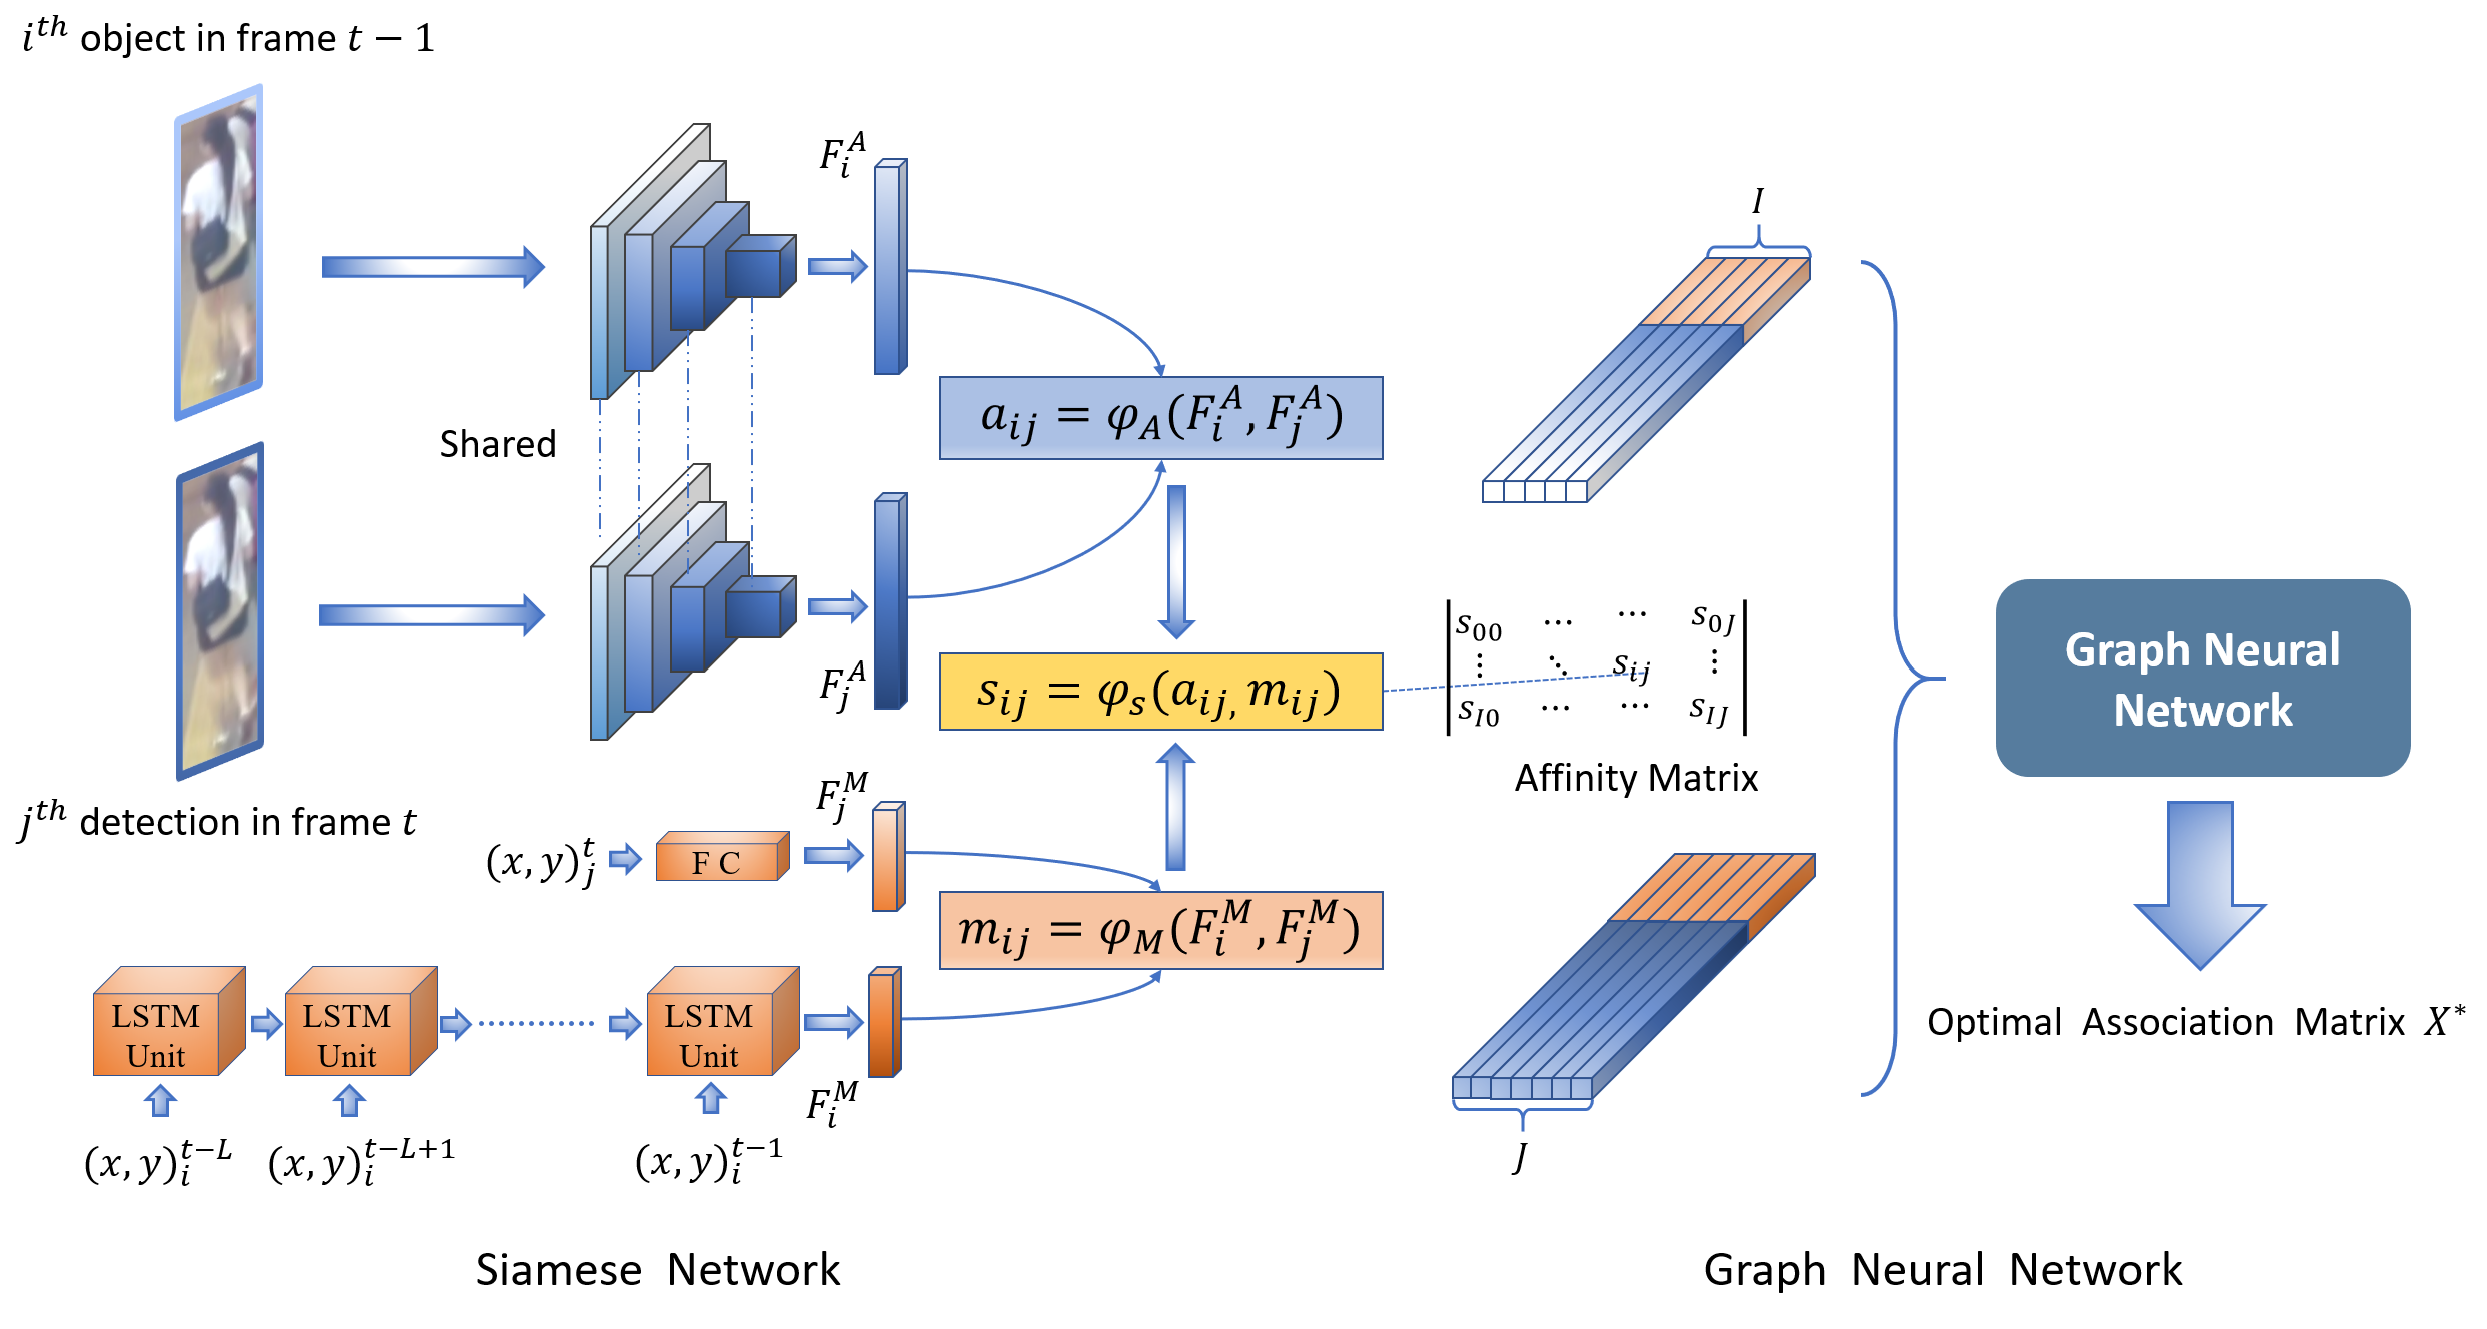
\includegraphics[width=5.4in]{figures/C2Fig/pipeline.pdf}
	\caption{
		类脑视觉目标跟踪的网络架构
	}
	\label{fig:c2:pipeline}
\end{figure*}

\subsubsection{视网膜和背侧/腹侧通路}

视网膜上的空间选择器为当前帧 $F_t$ 选择中央凹视图 $f_t$,它的输出被输入到两条相互连接的腹侧/背侧通路。
腹侧通路识别被跟踪的目标,而背侧通路学习被跟踪目标的运动特征。
% 引入非局部注意力机制。(自上而下的注意力)
腹侧/背侧通路中的外观注意力由当前帧自下而上的中心凹视图信息 $f_t$ 和前一帧自上而下的外观注意力信息 $\alpha_{t+1}$ 所驱动。
然而,中央凹的空间注意力只依赖于空间注意力信息 $a_{t+1}$,
在这种情况下,自下而上的信息仅具有局部影响并依赖于某个位置的显著性输入,
但自上而下的信息将全局特征结合到局部分析中~\cite{attention}。
%


%背侧通路中的神经元将显著目标 $d_t$ 和中央凹视图中的背景进行分割。
%使用精调后的表征 $m_t$ 计算工作内存 $h_t$。


(1) \textbf{视网膜}: 
在类脑模型的处理流程中,根据空间注意力机制~\cite{ratm} 进行建模。
对于输入帧 $F_t \in R^{W \times H}$ 形成矩阵 $M_t^x \in R^{w \times W}$ 和 $M_t^y \in R^{h \times H}$,
矩阵中的每一行都包含一个高斯分布。
高斯分布的位置和宽度决定了输入帧的哪些部分被选为视网膜中的中央凹视图 $f_t$。
因此,中央凹视图 $f_t \in R^{h \times w}$ 可以表示为:
\begin{equation}
f_t = M_t^y F_t (M_t^x)^T \mbox{,}
\end{equation}
用连续矩阵行的分布中心、步长和方差来表示注意力。
与循环注意力跟踪类似~\cite{hart},只有步长和分布中心是通过 LSTM 预测的,而方差依赖于步长。
该操作在估计较小的方差时避免了过度的偏差,有助于提高学习的速度。
此外,中央凹 $f_t$ 的大小依赖于具体的实验分析。


(2) \textbf{腹侧通路}: 
%初级视觉皮层 V1 和腹侧通路学习外观表征 $v_t$,
腹侧通路(包括初级视觉皮层 V1)将中央凹视图 $f_t$ 转换为固定维度的外观表征向量 $v_t$,其中包括被跟踪目标的空间特征和外观特征,
具体地网络结构依赖于具体的实验分析。
在本章的腹侧通路架构中,使用卷积神经网络实现初级视觉皮层 V1,这是腹侧通路和背侧通路共享的模块。
然而,通常使用若干个卷积层和最大池化层来实现模仿人类初级视觉皮层 V1~\cite{theoretical_neuroscience}。
%这些层模仿人类的 V1~\cite{theoretical_neuroscience},并与背侧通路共享。
在这以后,处理流程分为背侧通路和腹侧通路。
最后,通过卷积神经网络提取被跟踪目标的特征 $v_t$,以实现腹侧通路功能。

(3) \textbf{背侧通路}: 
背侧通路(包括 V1 和 MT/MST)用于提取运动特征,将显著目标 $d_t$ 和中央凹视图中的背景进行分割。
%并计算中央凹视图的前景分割 $d_t$。
使用动态滤波网络~\cite{brabandere2016dynamic} 建模背侧通路(MT/MST),用于处理中央凹视图前景和背景之间的空间关系。
%背侧通路(包括 V1 和 MT/MST)中的神经元将显著目标 $d_t$ 和中央凹视图中的背景进行分割。
%使用精调后的表征 $m_t$ 计算工作内存 $h_t$。
FC$(\cdot)$ 表示全连接层,
所以 MT/MST 中基于外观表示 $\alpha_t$ 动态预测卷积滤波器 $\phi_t$ 为:
\begin{equation}
\left\{ \phi _t ^i \right\}_{i=1}^N = \text{FC}(\alpha_t) \mbox{,}
\end{equation}
V1 输出的的特征经过具有 $N$ 个卷积层的非线性滤波器,
然后,将其输出传递给卷积核大小为 $1 \times 1$ 的卷积和 Sigmoid 激活函数,将特征转换为二维掩码 $d_t$。
$d_t$ 中的每一点都表示被所跟踪目标占据的概率。

背侧通路的位置图是基于腹侧通路抽取的目标表示,这模拟了视觉系统中的噪声抑制机制。
因为在当前帧没有跟踪目标的表征时,LSTM 中的目标表征不会被覆盖,所以使用这种机制可以处理遮挡和漂移的情况。
因此,腹侧和背侧通路的输出可以被整合为:
\begin{equation}
m_t = \text{FC}(conc(v_t \odot d_t)) \mbox{,}
\end{equation}
其中 $\odot$ 表示通过特征掩码执行显著目标提取的哈达玛积,
$conc$ 表示将矩阵的所有行连接成向量的连接运算符。


\subsubsection{额叶视区}
所提出的类脑跟踪方法性能取决于估计下一帧中目标外观和位置的能力。
因此,它在很大程度上依赖于跟踪目标状态的预测。
而 LSTM 可以利用时空和外观特征,使所提出的模型能够处理遮挡和漂移的情况,例如跟踪目标被其他干扰物遮挡的情况。

如图~\ref{fig:c2:pipeline} 所示,将 LSTM 模块命名为 FEF,利用输出误差来预测眼球运动。
在平滑跟踪中,FEF 区域接受来自腹侧/背侧流的输出 $m_t$,
精调后的目标表征 $m_t$ 用于更新 FEF 中的隐藏状态 $h_t$,
并在 FEF 中存在类似的预测动作~\cite{b11,b13,b14}。
当模型训练过程中,被跟踪目标和眼球运动之间的延迟减少时,输出误差趋向于零。
因此,LSTM 需要即使在没有图像输入的情况下依然能够推断眼球的运动。
\begin{equation} \label{equ:c2:LSTM}
h_t, o_t = \text{LSTM}(h_{t-1}, m_t) \mbox{。}
\end{equation}


\subsubsection{脑干和小脑}
脑干和小脑一起(包括脑桥核、绒球、小脑蚓体和前庭核)使用全连接层进行建模,
%以产生注意力 $a_{t+1}$,外观 $\alpha_{t +1}$,以及眼位校正信号 $\Delta p$,
%甚至最后通过动眼神经生成眼球运动信号 ($\Delta p_t$) 。
然后利用背侧流的输出 $d_t$ 和额叶视区的输出 $o_t$ 来估计注意力 $a_{t+1}$ 和外观 $\alpha_{t+1}$,
最后通过动眼神经生成眼球运动信号 $\Delta p_t$。
\begin{equation} \label{equ:c2:FC}
\Delta p_t, \Delta a_{t+1}, \alpha_{t+1} = \text{FC}(conc(d_t), o_t) \mbox{,}
\end{equation}
\begin{equation} \label{equ:c2:attention}
a_{t+1} = a_t + tanh(c) \Delta a_{t+1} \mbox{,}
\end{equation}
其中 $c$ 是一个可训练参数,用较小的值进行初始化以限制训练期间模型更新的大小。
方程~\ref{equ:c2:LSTM} 到 ~\ref{equ:c2:attention} 描述信息更新的过程。
通过累积注意力变化来计算眼睛注视的位置,
如章节~\ref{sec:loss} 所示,学习空间注意力来估计下一帧中被跟踪目标的位置,并预测在时间 $t$ 相对于注意力的注视位置 $p_t$。
\begin{equation}
p_t = a_t + \Delta p_t \mbox{。}
\end{equation}

此外,参考脑干和小脑都可以利用反向动力学控制器进行建模的发现和想法~\cite{b9,purkinje_IDC},
基于动力学的平滑跟踪模型~\cite{b9},这里假设反向动力学控制器是完美的,因此眼球的运动信号可以表示为:
\begin{equation}
\Delta p_t = \Delta p \mbox{,}
\end{equation}
其中 $\Delta p$ 是眼球运动的低通滤波器。
基于这个假设,在该研究中不需要实现反向动力学控制器。



\subsection{损失函数} \label{sec:loss}
可以通过优化一组损失来训练所提出的 BTN,包括跟踪损失、背侧/腹侧流损失和辅助损失。
BTN 损失 $L_{b}$ 由下式给出:
\begin{equation}
L_{b} = L_t + L_d + L_v + L_a \mbox{。}
\end{equation}
BTN 损失的详细信息如下所述。

\subsubsection{跟踪损失}
为了达到视觉跟踪的目的,即定位目标在当前帧的位置,损失函数第一项采用预测的边界框和真实边界框之间的交并比。
由于交并比对目标和图片尺寸具有不变性,用它来衡量定位跟踪目标的准确性是比较适合的。
虽然交并比不对应任何概率分布并且不能被归一化,但它经常用于跟踪性能的评估~\cite{vot2016}。
同时,使用交并比的交叉熵损失函数代替传统的 L2 损失函数是由于目标定位使用 L2 损失的一个缺点是会使模型在训练过程中更偏向于尺寸更大的物体,因为大目标的 L2 损失更容易大于小目标。
所以在这里根据 UnitBox~\cite{unitbox} 将跟踪损失 $ L_t $ 表示成交并比的负对数:
\begin{equation}
L_t = -\log(\mbox{IoU} ( \frac{p_t \cap \hat{p}_t}{p_t \cup \hat{p}_t} ))\mbox{。}
\end{equation}

\subsubsection{背侧流损失}
使用背侧流中的空间注意力机制从视频帧中挑选出被跟踪的目标。
为了估计该模块的参数,跟踪系统必须预测目标的运动,而这个预测过程很难恢复原状。
使用两项背侧流损失来保证随着关注目标区域的减少,跟踪的精度会上升。
背侧流损失 $ L_d $ 的第一项限制了预测的注意力区域尽可能地覆盖目标的边界框,
而第二项防止注意力区域变得太大(最大为整个输入帧的大小),这里的对数操作是为了适当的裁剪以避免数值不稳定。
\begin{equation}
L_d = -\log (\frac{a_t \cap p_t}{p_t}) - \log (1 - \frac{a_t \cap F_t}{a_t \cup F_t})\mbox{。}
\end{equation}

\subsubsection{腹侧流损失}
当被跟踪目标(比如一个特定的行人)是动态开放环境中时,设置腹侧流中外观注意力的目的是为了抑制干扰。
为了达到这个目的,在外观注意力上设置一个损失函数以选出被跟踪的目标。
给定注意力区域 $a$ 和边界框 $p$,% (x,y,w,h)
记 $r(a_t, p_t): R^4 \times R^4 \rightarrow \left\{0,1\right\} ^{h_v \times w_v}$ 为目标函数,
输出一个和 V1 的输出一样大的二进制掩膜。
该掩膜就叫做显著目标区域 $g$,其中边界框和显著目标重叠的位置值为 1,其他地方为 0,也就是只保留下边界框中包含目标的像素。
%如果将交叉熵记作 $H(p, q) = -\sum_{z} p(z)\log q(z)$,那么
腹侧流损失函数可以表示为显著目标区域的预测值和前背景分割的真实值之间的交叉熵:
\begin{equation}
L_v = - r(a_t, p_t) \log(d_t)\mbox{。}
\end{equation}

%\subsubsection{正则化项}
%对模型的参数 $\theta$ 和动态参数的期望值 $\phi_t(\alpha_t)$ 应用 L2 正则化,表示为:
%\begin{equation}
%L_u = 
%\frac{1}{2} \left\vert \left\vert \theta \right\vert \right\vert _2 ^2 + 
%\frac{1}{2} \left\vert \left\vert \phi_t \right\vert \right\vert _2 ^2 .
%\end{equation}

\subsubsection{辅助损失}
对模型的参数 $\theta$ 和动态参数的期望值 $\phi_t(\alpha_t)$ 应用 L2 正则化。
同时为了避免超参数调优,参考多任务学习~\cite{multitask}来学习各个损失的权重 $\lambda$。
使用全为 1 的向量初始化权重后,给损失函数添加正则化项,则辅助损失 $L_a$ 可以表示为:
\begin{equation}
L_a = 
\frac{1}{2} \left\vert \left\vert \theta \right\vert \right\vert _2 ^2 + 
\frac{1}{2} \left\vert \left\vert \phi_t \right\vert \right\vert _2 ^2
- \sum_{i} \log (\lambda_i^{-1})\mbox{。}
\end{equation}




\section{大脑数据分析}
为了比较 DNN 的视觉目标跟踪和人脑平滑跟踪的相似性,首先需要从各种眼球运动中提取平滑跟踪,然后选择相应的大脑区域和激活用于相似性计算。

\subsection{视频刺激的运动估计}
由于平滑跟踪行为和视频中目标的移动高度相关,首先使用计算机视觉方法对所有视频帧的运动进行估计。
尽管目前已存在许多精度高的运动估计算法,但仍然会产生额外的噪声输出,所以这里使用两种不同的算法来增强运动估计的鲁棒性。
% 孔径问题:从小孔中观察一块移动的黑色幕布观察不到任何变化。但实际情况是幕布一直在移动中。(人类的视觉系统在局部观察时有孔径问题)
% 解释:https://blog.csdn.net/dengheCSDN/article/details/81747063
% 根据结构张量能区分图像的平坦区域、边缘区域与角点区域(https://www.cnblogs.com/revere7/p/9705956.html)
第一种算法是仅对孔径问题不敏感的点(比如角点)进行运动估计,以提供稀疏光流场并估计运动~\cite{structure_tensor}。
首先对输入视频做采样因子为 2 的空间二次抽样,然后创建一个拥有五个空间层和两个时间层时空高斯金字塔。
对于这些多尺度表征的每一层,计算每个像素的运动速度。
对速度的估计值相对于原始视频分辨率进行正则化,并以类似于金字塔合成的方式合并到处理流程当中~\cite{pyramid_synthesis},并对过高的速度值使用对应速度的百分之九十进行裁剪。
第二个算法使用基于光流计算的插值方法~\cite{epicflow}。
该算法首先使用边缘保持插值的稠密匹配,然后进行能量最小化操作。
%一个EpicFlow算法估计运动的例子如图~\ref{fig:gaze_traces}b所示。
最后使用这两种算法,计算出每个视频帧像素偏移的平均长度。

%\begin{figure*}[ht]
%	\centering
%	% 导入.pdf垂直显示?
%	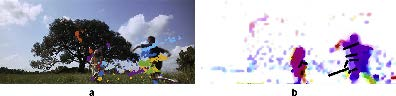
\includegraphics[width=6in]{./figures/C2Fig/gaz_traces.jpg}
%	\vspace{0.2em}
%	\caption{平滑跟踪存在性演示和计算。
%		(a)对于受试位于核磁共振扫描仪中观看 StudyForrest 数据集,叠加凝视轨迹的样例帧(超过400ms的时段;每个颜色对应一个受试)。
%		通过被拉长的点云可以证明平滑跟踪是存在的。
%		(b)使用EpicFlow算法计算光流。
%		估计的运动(黑线)和视频中实际的运动对应得很好。
%		黑线表示“多观察者平滑跟踪(MOSP)”算法的输出(比如在400ms的时间窗口中自动检测平滑跟踪片段)。
%		} 
%	\label{fig:gaze_traces}
%\end{figure*}


\subsection{平稳跟踪样本的提取}
实验中每个凝视样本都包含一个四元组:时间、显示器坐标系下的横坐标 $x$ 和纵坐标 $y$、眼跟踪质量的置信度估计。
因为数据集使用的是单眼跟踪,所以置信度为 1 表示好的眼跟踪,而 0 表示跟踪丢失。
经数据检查后发现在所有受试中跟踪丢失的比例一般在 $1.2\%$ 和 $16.7\%$ 之间,而受试 5 和受试 20 跟踪丢失特别明显,丢失比例分别是 $86.7\%$ 和 $39.0\%$,所以将他们的数据从分析中剔除。
%
对余下的凝视样本利用一种比较有代表性的基于密度的聚类算法 MOSP~\cite{mosp,mosp_imp} 进行分类以得到平稳跟踪样本。
该算法在手动标注的公共数据集上和几个最新的眼动检测算法~\cite{fix_sp_det,remodnav} 相比有很好的分类性能。
MOSP 算法的另一个优势是在程序中使用了简单且容易理解的门限值,这样保证在使用过程中比较容易进行调整,而不像一些深度学习方法~\cite{auto_classification,gazenet} 的超参数调整困难。
这一步 MOSP 取得较高的平滑跟踪检测精度(比如较低的误检)对后续的分析非常重要。

MOSP 算法包括两个步骤,第一步负责眼跳检测,先将眼跳剔除,第二步负责区分注视和平滑跟踪。
眼跳检测算法~\cite{var_natural} 使用一个高速度门限值和一个低速度门限值。
眼跳检测器使用高速门限值进行初始化,然后往门限值两端进行扩展,直到小于低速门限值。
使用大于输入样本之间噪声的高速门限值使算法对噪声更加鲁棒。
MOSP 算法的第二步是进一步处理眼跳间的间隔,通过给几乎可以确定是注视的样本赋予一个注视的标签。
余下的样本就标记为平滑跟踪的候选结果,并在所有受试中进行处理。
然后,只有当凝视样本密度大于某个门限值时才使用基于密度的聚类算法 DBSCAN 进行聚类。
基于密度的聚类算法能很好地检测出平滑跟踪是因为平滑跟踪的的两个属性。
% 
首先,只有在给定时间内刺激出现运动时,平滑跟踪才会出现;并且视频刺激中每一帧移动的目标数目较少。
%
第二个特点是移动的目标能吸引受试的注意力(特别是在电影中),并且它们经常会被超过一个受试所跟踪。
%MOSP算法输出和聚类的示例如图~\ref{fig:gaze_traces}所示。
平滑跟踪的这两个属性使算法能够把真实的平滑跟踪从漂移和类平滑跟踪中区分开来,这对于 fMRI 实验中的平稳跟踪样本的提取特别重要。
%(因为他们比实验室记录有更高的噪声)。
即使一些凝视样本被错误的标记成候选平滑跟踪,只要在当前时间的相同区域其他受试没有相同的模式,那么它也不会被标记成平滑跟踪,通过这些机制提高算法的鲁棒性对识别与处理平滑跟踪相关的大脑区域特别重要。
%然而当没有足够受试跟踪一个目标时,可能会有丢失一些平滑跟踪的缺点(即降低对平滑跟踪的敏感性),增长的特异性对识别与处理平滑跟踪相关的脑区特别重要。

由于原始的 MOSP 算法是针对 GazeCom 数据集~\cite{var_natural} 进行设计和优化的,在本实验中对一些参数与进行了调整。
%(参见在线数据的完整详细信息)。
因为增加凝视轨迹的数目会提高平滑跟踪检测算法的精度,所以同时使用了不在核磁共振扫描仪里的记录(获取难度较小,且相比于扫描仪记录有更少的噪声)和在扫描仪里的记录。
% 观测角中每一度应该包含大约相同的像素
尽管刺激大小不同,对不在扫描仪里的记录使用单位观测角中所包含的像素数来进行按比例缩放;
所以使用两个数据集进行平滑跟踪片段检测会有更高的置信度。
%(2秒间隔下共有的平滑跟踪为0.84的$r^2$)。


\subsection{核磁共振数据分析}
本实验使用 SPM12 工具进行核磁共振数据的分析。
首先对每个 fMRI 记录利用标准的处理流程进行预处理~\cite{mri_analysis}。
包括对每个会话的平均图像进行功能性数据对齐(由于公开数据集已经做了时间校正,在这里就没有使用间时间校正),并将对齐后的数据与大脑解剖的 T1 扫描进行配准,
%\footnote{使用头动校正处理不同扫描之间体素对应关系的不一致,导致血液动力学响应被头动引起的信号所淹没。},
然后将其正则化到 MNI 模板,再重采样到 $3 \times 3 \times 3$立方毫米的体素中。
最终,在脉冲的半峰全宽上使用 8 毫米高斯核进行平滑。

在 StudyForrest 数据集的记录中,将整部电影刺激分割成 8 个不同的视频片段,每个大约 15 分钟,在扫描仪中分别展示给每个受试。
在第一阶段的个体分析中,
%(个体内的分析,8 个电影片段之间的分析),
为了建模整个《阿甘正传》电影,将 8 个记录会话组合到一个设计矩阵中,每一行表示一个电影片段。
在设计矩阵的每个会话中,从同一受试观察不同的电影片段的凝视中回归出一个平滑跟踪回归变量、一个眼跳回归变量和一个电影运动回归变量。
为了考虑受试之间血液动力学响应开始时刻和宽度的变化,沿着时间和离散度梯度方向使用标准血液动力学响应函数(Hemodynamic Response Function,HRF)。
除了以上三个回归变量,还使用了从预处理重对齐步骤中得到的六个头部运动分量\footnote{3个平移分量($x$、$y$、$z$)和3个旋转分量} 作为用于校正的干扰因素回归变量。

为了和扫描仪重复时间相一致,眼动和运动回归变量建模成有 2 秒间隔的事件序列,因此每个事件都被表示成两个扫描之间变化的回归变量。
% 幅值为跟踪点在fMRI上的影响范围?
% 幅值从0增加到1(相当于减了一个平均值?)
每个事件的幅值都根据 2 秒时间窗口内对应的眼动或运动数目进行调整,当和整体均值相同时对应的值为 0。
%,并线性增长到最大值1。
回归建模的详细描述在下一节~\ref{sec:regressor_modelling} 中给出。
%随着回归变量如何建模变得明显,
在回归变量建模中,如果没有创建两个之间的强烈的正相关或者负相关,就不可能同时建模注视和平滑跟踪。
为了使注视和平滑跟踪相互依赖更加清晰,可以考虑受试开始跟踪一个目标。
然后随着注视幅值的减少,平滑跟踪回归变量的幅值就会成比例增加。

对每个受试数据独立地应用广义线性模型后,使用每个回归变量血液动力学响应函数的幅值部分(为了计算和平滑跟踪相关的感兴趣部分进行对比,该处理过程横跨了对应 8 个电影片段的 8 个记录会话)。
这些对比包括眼动和运动主要响应的对比、平滑跟踪和眼跳之间的对比,以及眼动和运动的对比。
最后,在第二阶段受试之间核磁共振分析中,对 13 个有效受试的第一阶段对比结果进行单样本 $t$ 检验。
%聚类结果(使用$p$值小于0.001的初始门值校正情况下,$p$值小于0.05的多重比较谬误)覆盖在三维大脑模型上,并在实验和结果章节~\ref{sec:c2:results} 进行展示。

\subsection{回归变量建模} \label{sec:regressor_modelling}
如上节所述,回归变量并不是对每个眼动事件单独地进行建模,而是把它置于 2 秒时间间隔内,根据所在时间窗口中每种眼动的数目进行调制。
在该实验中将电影本身运动考虑进来,在连续 2 秒的时间窗口内通过电影运动的均值来进行调制。
%
具体来说,将眼动调制参数量级的计算加以考虑,它有三个主要影响因素:
% 不同刺激,特定功能(平滑跟踪)在同一受试之间激活的平均效果
% 为了得到实时的sp响应,不进行不同刺激的回归?
\begin{enumerate}
	\item 捕获不同刺激之间眼动的差异,并通过每个受试的每种眼动平均百分比表现出来,这等同于不同观察行为的平均。
	
	% 不同眼动类型 方差不同
	% (方差越大,眼动调制强度越小)
	\item 捕获分布上的差异和不同眼动之间的方差,这是一个常数,且眼动调制强度和方差成反比。
	为了保证有 $95\%$ 的调制值在 1 以下,调制因子从数据中进行选择。
%	(如图~\ref{fig:sp_ratio}所示)。
	% $m_{sac}$
	由于与眼跳相关的不同输入刺激拥有较小的方差,因此将眼跳的调制值设置为 1.5。
	% 拉近两者的分布
	% $m_{sp}$
	为了反映平滑跟踪时眼睛运动中较大的方差,将平滑跟踪的调制值设置为 5 ,当没有移动目标时候,平滑跟踪不会出现,而当存在一个显著移动的目标时,平滑跟踪能够执行较长一段的时间。
	
	%% 不同的受试(二层次分析)
	\item 捕获不同受试之间的变化。
	特定受试的基本要素是基于每个眼动的观察,如果受试之间眼动存在较大不同,可能会直接或间接导致所得到的大脑连接性的不同~\cite{mueller2013individual,vanderwal2017individual}。
\end{enumerate}
%(1)第一个因素是捕获不同自然刺激之间眼动的差异,并通过每个受试的每种眼动平均百分比表现出来,这等同于不同观察行为的平均。
%(2)第二个因素是捕获分布上的差异和不同眼动之间的方差,它们是一个常数,眼动调制强度和方差成反比(方差越大,眼动调制强度越小)。
%为了保证有$95\%$的调制值在1以下,因子从数据中进行选择(如图~\ref{fig:sp_ratio}所示)。
%由于与眼跳相关的不同输入刺激拥有较小的方差,因此眼跳的调制值$modulation_{sac}$设置为1.5。
%% 拉近两者的分布
%为了反映平滑跟踪眼睛运动中较大的方差,将平滑跟踪的调制值$modulation_{sp}$设置为5,当没有移动目标时候,平滑跟踪不会出现,但是当一个显著移动目标存在时,平滑跟踪能够执行较长一段的时间。
%% 不同的受试(二层次分析)
%(3)第三个因素是捕获不同受试之间的变化。
%特定受试的要素是基于每个眼动的普遍性观察,受者试之间的不同,可能会直接或间接导致大脑连接性的不同\cite{mueller2013individual,vanderwal2017individual}。
%在 StudyForrest 数据集的案例中,不同受试之间眼跳的变化从$5.8\%$到$12.4\%$,平滑跟踪的变化从$11.5\%$到$19.3\%$。
%因此,如果使用总平均值,一些受试的相关激活会被抑制,一些又会被放大。

在 StudyForrest 数据集中,不同受试之间眼跳所占的比例从 $5.8\%$ 到 $12.4\%$,平滑跟踪所占的比例从 $11.5\%$ 到 $19.3\%$。
因此,如果使用总平均值,一些受试的相关激活会被抑制,一些又会被放大。
%比如对于一个假想的受试,他在全部实验中,平滑跟踪所占的百分比为 $overall_{sp}=15\%$,并在给定的片段有 $clip_{sp}=10\%$ 不执行平滑跟踪。
%现在在一个2秒时间窗口中 $window_{sp}=85\%$ 的间隔被标记为平滑跟踪,
%% 实际执行平滑跟踪的比例为:85%-10%
%这时候调制强度
%\begin{equation} \label{equ:modulation_sp}
%modulation_{sp} = \frac{window_{sp}-clip_{sp}}{m_{sp} * overall_{sp}} = \frac{85\%-10\%}{5*15\%} = 1
%\end{equation}
%根据公式~\ref{equ:modulation_sp} 
在数据集中所有 2 秒间隔内计算调制参数后,发现平滑跟踪回归变量和眼跳回归变量之间的皮尔逊相关系数 $r=0.02$,这很好的表明了两者之间不相关且没有共享的可变性。

同理对于运动估计调制参数遵循和眼动参数建模相似的流程。
并且,这里对于每个刺激通过平均运动的内容来捕获他们的稳定状态。
在所有刺激片段中,结果值根据运动值的 90\% 进行正则化,并将结果的最大值限制到 1,以较少离群值的影响。


% 表明眼跳比平滑跟踪一些
%\begin{figure*}[ht]
%	\centering
%	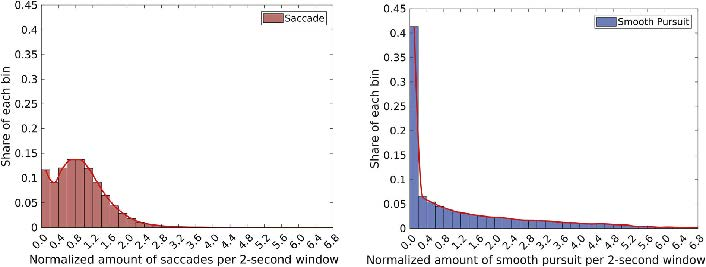
\includegraphics[width=6in]{./figures/C2Fig/sp_ratio.jpg}
%	\vspace{0.2em}
%	\caption{当进行事件相关的个体层次分析时,在2秒时间窗口内检测出来的眼跳(左)比例的概率分布和平滑跟踪(右)比例的概率分布,正则化的目的是为了使每个受试的均值为1。
%	更陡峭的分布表示不同受试和时间之间有更高的可变性。
%	眼跳的比例(红色)有更低的可变性,并且是以1为中心。
%	平滑跟踪(蓝色)有更大的可变性,其峰值接近于0表示有较少的平滑跟踪(比如场景中没有平滑跟踪的目标)。
%	} 
%	\label{fig:sp_ratio}
%\end{figure*}


%\subsection{额外用于验证的回归变量}
除了平滑跟踪和眼跳的回归变量,本实验还使用了运动回归变量用于建模视频中的全局运动,
并进一步探索了两种变化,
第一个是运动建模的变化,通过凝视位置周围的窗口来获得运动的局部估计,
第二个是在相同的窗口为了和视网膜上运动相似,从平均上下文速度中抽取平滑跟踪的速度。
%由于局部运动的结果低于全局运动水平,所以我们没有在结果章节中说明,而是在后面讨论部分讨论它。
为了进一步理解是什么驱动了眼睛运动,也将场景动态开放性和边缘密度估计的模型作为额外的回归变量,这些被调制值等同于之前描述的运动回归变量。
使用标准显著性模型来计算场景动态开放性,作为每一帧的显著性熵~\cite{itti1998a}。
与图像显著性熵类似,边缘密度在拉普拉斯金字塔的第三层作为每一帧绝对像素值的熵,它表示每度大约 3-6 个循环空间频率范围中的边缘,接近人类对比敏感函数的峰值。
%同时这些结果在后面都会讨论。



% ref: Brain-Score: Which Artificial Neural Network for Object Recognition is most Brain-Like? -> Bran Benchmarks
\section{评价指标:类脑跟踪分数}
这一部分介绍了衡量深度神经网络模型与人类大脑皮层之间的相似性的类脑跟踪分数 BTS。
BTS 是在特定实验数据集上测试的指标,包括眼动行为预测性和皮层神经预测性两个指标。

为了获得关于大脑相似性的量化指标,参考开源平台 Brain-score~\cite{SchrimpfKubilius2018BrainScore} 并提出了 BTS,这是一个设计良好的用于评估跟踪模型类脑预测能力的指标:
(a) 对于 StudyForrest 数据集的每个输入视频帧,预测人眼跟踪目标时的平均人眼运动~\cite{gaze_forrest};
(b) 在 StudyForrest 数据集~\cite{gaze_forrest} 上预测人类视觉区域 MT/MST 中大脑皮层位置对每个输入视频帧的平均激活响应。
%所有眼动的娇娇
为了在统一指标上评估 BTN,该指标计算了眼动行为预测性指标和皮层神经皮层预测性指标的平均值。

\subsection{眼动行为预测性}
眼动行为度量的目的是衡量对于特定任务深度神经网络输出与人眼行为输出之间的相似性~\cite{rajalingham2018large}。
在人眼目标跟踪中,被试者的注意力是一个与人瞳孔有关的圆形范围。
因此,将模型呈现的行为模式(眼睛注视的位置和瞳孔的大小)建模为圆形,并且它不同于视觉目标跟踪中的长方形边界框。
同时,由于该工作不仅仅是为了提高计算机的跟踪性能~\cite{schrimpf2020integrative},更主要目的是实现类人的智能;
如果 BTN 获得了更好的行为相似性,就可以很好地预测眼睛注视的位置和范围。
否则会导致深度神经网络获得了完美的边界框拟合,却无法获得良好的人眼行为预测效果。

如表~\ref{fig:c2:introduction} 所示,使用的 12 个视频序列是在自然背景下有一个显著的目标在移动,每个视频序列大约 20 秒,并利用眼动仪记录下受试的注视范围来表示跟踪显著目标,
并使用 12 个图像序列中的 149 张图像的受试眼球运动和深度神经网络预测来分析和评估所提出的模型的眼动行为预测性能。
总共的 149 帧图像中,每一帧都作为深度神经网络的输入,用于预测眼睛的注视范围。
然后通过每一帧中眼睛注意力的范围来衡量这种眼动行为预测性。

目标跟踪深度神经网络的输出结果是所跟踪目标的边界框,而受试的注意力是一个包含中心坐标 $x$、$y$ 和半径的圆形范围。
因此将眼动预测性或行为评分建模为实际眼睛注意的圆形范围 $S_{roi}^a$ 与深度神经网络预测边界框 $S_{roi}^b$ 之间的交并比(Intersection over Union,IoU),
并将所有帧序列中的整体行为指标~$s_b$ 作为眼动预测分数:
\begin{equation}
s_b=\frac{area(S_{roi}^a \cap S_{roi}^b) }  { area(S_{roi}^a \cup S_{roi}^b) } \mbox{。}
\end{equation}


\subsection{皮层神经预测性}
皮层神经预测性是指在源系统中(比如深度神经网络)评估给定输入图像 $X$,预测在目标系统(比如视觉区域 V1 和 MT/MST)中的激活响应。
作为输入,该度量方法的评估过程为:刺激 $\times$ 神经网络 = 激活响应,这里的神经网络可以是深度人工神经网络,也可以是灵长类的大脑皮层。
并且源神经网络(深度人工神经网络)可以使用线性变换映射到目标神经网络(灵长类皮层网络):
\begin{equation}
y = Xw + \epsilon \mbox{,}
\end{equation}
这里 $w$ 表示线性回归的权重,$\epsilon$ 表示皮层记录的噪声。

实验中呈现给 13 个受试的 149 帧图像包括在自然场景中出现的显著跟踪对象,并且记录下 MT/MST 体素中的 2177 个神经响应。
此外还展示了 BTN 中最具预测性的网络层和特定的模型区域。

在本实验中,这些关系被拟合为从深度神经网络到大脑皮层的映射,并用这个映射关系来预测人的大脑皮层对视频帧的响应。
由于大脑的激活响应数据维度远远大于神经网络模型激活数据的维度,所以利用主成分分析(Principal Component Analysis, PCA)~\cite{2002Principal} 将大脑激活维度压缩到指定的维度来进行程序运行加速和相关性分析,
并利用来自 MT/MST 的激活来进行拟合。 
最终使用皮尔逊相关系数 $s_r$ 来衡量最终人工神经网络模型和视觉运动皮层的神经相似性分数,如下所示:
\begin{equation}
s_r=\frac{\sum_{i=1}^{n} (y_i-\bar{y}) (y_i^\prime - \bar{y}^\prime) }{\sqrt{\sum_{i=1}^{n} (y_i - \bar{y})^2 (y_i^\prime - \bar{y}^\prime)^2 }}\mbox{,}
\end{equation}
其中 $y^\prime$ 是人工神经网络模型特定层的激活,$y$ 是人类大脑皮层特定区域的激活,$n$ 是深度神经网络中对应的特征维度,$\bar{y}$ 和 $\bar{y}^\prime$ 是所有神经响应值的中位数(使用中位数是因为响应通常是非正态分布)。

\subsection{总分数}
为了全面衡量 BTN 的类脑性能,同时考虑了 IoU 行为度量和 MT/MST 皮层度量。
下面给出的 BTS $s_{t}$ 是两个分数的平均值 :
\begin{equation} \label{equ:score_btn}
s_{t} = \frac{s_b + s_r}{2}\mbox{。}
\end{equation}
考虑到归一化可能会惩罚方差较小的分数,而应该平等对待两个分数对 BTS 的重要性程度,因此 BTS 的设计没有在各个分数大小上进行归一化。

%映射步骤在多个训练-测试图像刺激集的划分中执行。
%每次运行时,使用训练图片学习的权重将源神经网络的输出映射到目标神经网络的响应,然后使用这些权重来与剩余图像的响应$y'$。
%我们分别使用MT和FEF的神经元响应来计算映射权重的拟合。
%为了获得每个神经网络的神经预测性,将预测的响应$y'$和测量的皮层神经网络响应$y$进行比较来计算皮尔逊相关系数$r$(评估两个连续变量之间的线性关系):
%\begin{eqnarray}
%r = \frac{\sum_{i=1}^{n}(y_i^\prime - \bar{y})(y_i^\prime - \bar{y})}
%{\sqrt{\sum_{i=1}^{n} (y_i - \bar{y})^2 (y_i^\prime - \bar{y}^\prime)^2}}
%\end{eqnarray}
% study: https://blog.csdn.net/qq_30081043/article/details/107154233

%使用所有单个神经网络预测值的中位数(比如在目标脑区所有测量的目标位置)来获得训练-测试集切分的预测性分数(使用中位数是因为响应通常是非正规分布的)。
%最终目标脑区的神经预测性分数为所有训练-测试集切分的平均值。
%
%我们进一步通过将相同图像的重复表示划(一个是深度人工神经网络的响应,一个是皮层神经网络的响应)分为两半,来估计神经响应之间的内部一致性,并计算每个神经网络两个划分之间的Spearman-Brown-corrected的皮尔逊相关系数。

%在实际实现中,我们发现对于源系统(深度人工神经网络)中的高维度,标准的线性回归方法相对较慢,并且鲁棒性不够。
%因此我们使用25个部件的偏最小二乘(PLS)回归\cite{performance_optimized}。
%我们通过先将源特征(深度人工神经网络的特征)使用主成分分析(PCA)投影到更低维度的空间。
%投影矩阵是图片集一个选择的特征中获得,所以在训练-测试集切分中该投影是不变的。
%然后投影矩阵用于转换源神经网络输出的特征。
%结果显示对1000个验证图片特征响应的每一层,从特征响应中获得了1000个主成分。
%该1000个主成分就捕获了源模型的最大的方差信息。

%\subsection{fMRI记录}
%目前使用的皮层响应数据记录是观察电影《阿甘正传》时的核磁共振数据\cite{gaze_forrest}。


\section{实验与结果分析} \label{sec:c2:results}
在这一节通过以下四个步骤说明所设计的 BTN 实验和其有效性。
首先,介绍了实验相关数据集和模型的具体实现。
其次,详细分析了眼动数据和对应的核磁共振数据。
然后,说明了 BTN 是一种有效的类脑跟踪模型。
最后,讨论了模型设计机制以及深度神经网络与神经科学的关系。


\vspace{0.6em}
\begin{table}[htbp]\wuhao
	\centering
	\caption{原始电影的分割和合并
	}
	\vspace{0.3em} 
	\begin{tabular} {c|cccc}
		%		{p{1.7cm}<{\centering}p{1.7cm}<{\centering}p{1.7cm}<{\centering}p{1.7cm}<{\centering}p{1.7cm}<{\centering}}
		%		\toprule[1.5pt]
		%		\hline
		\hline
		片段  & 开始时间  & 结束时间   & 开始帧 & 结束帧 \\ 
		\hline
		0   &00:00:00.00 &00:21:32:12 &0 &32,312  \\
		1   &00:24:13.24 &00:38:31.23 &36,349 &57,798   \\
		2   &00:38:58.20 &00:59:19.22 &58,470 &85,997   \\
		3   &00:59:31.17 &01:18:14.00 &89,293 &117,351   \\
		4   &01:20:24.16 &01:34:18.06 &120,616 &141,457   \\
		5   &01:37:14.19 &01:41:30.19 &145,869 &152,369   \\
		6   &01:42:49.19 &02:09:51.17 &154,244 &194,792   \\
		%		\hline
		\hline
	\end{tabular}
	\label{tab:movie_seg}
\end{table}


\subsection{数据集}
本研究所提出的 BTN 首先在具有挑战性 KITTI 数据集~\cite{kitti} 上进行训练。
该数据集包括 21 个视频帧序列,包括各种可能的干扰项。
此外,将这些序列中的 80$\%$ 作为训练数据集,20$\%$ 作为验证数据集。

为了测试和分析所提出的类脑模型,将公共数据集 Studyforrest ~\cite{gaze_forrest} 作为动态开放场景的代理。
在具体实验数据集中,使用 StudyForrest 来构建所使用的跟踪数据集~\cite{gaze_forrest}。
%\subsection{数据集}
从 StudyForrest 数据集所用的电影中抽取 12 个短视频(每个大约 20 秒)用于衡量计算机视觉跟踪和生物平滑跟踪的相似性。
为了和 fMRI 数据的采集频率保持一致,如表~\ref{tab:track_seg} 所示,所用的视频帧也采样间隔为 2 秒。
用手动的标注的方式提供人眼跟踪跟踪目标的真实边界框,用于评估计算机类脑视觉跟踪算法的精度。




\vspace{0.6em}
\begin{table}[htbp]\wuhao
	\centering
	\caption{所用到的 12 个视频片段详细信息}
	\vspace{0.3em}
	\begin{tabular} {c|cccc}
%		{p{1.7cm}<{\centering}p{1.7cm}<{\centering}p{1.7cm}<{\centering}p{1.7cm}<{\centering}p{1.7cm}<{\centering}}
%		\toprule[1.5pt]
%		\hline
		\hline
		跟踪段号  & 视频段号  & 开始帧   & 结束帧 & 图片数 \\ 
		\hline
		1     &3 &02:30.00 &02:48.00 &10  \\
		2   &4 &14:50.00 &15:14.00 &13   \\
		3   &5 &01:32.00 &01:48.00 &9   \\
		4   &5 &05:02.00 &05:20.00 &10   \\
		5   &6 &00:08.00 &00:24.00 &9   \\
		6   &6 &06:56.00 &07:10.02 &8   \\
		7   &6 &09:42.00 &09:56.01 &8   \\
		8   &6 &12:26.00 &12:44.00 &12   \\
		9   &7 &06:44.00 &07:06.00 &12   \\
		10  &7 &07:26.00 &08:28.00 &32   \\
		11  &7 &08:30.00 &08:52.00 &12   \\
		12  &7 &10:40.00 &11:10.00 &16   \\
%		\hline
		\hline
	\end{tabular}
	\label{tab:track_seg}
\end{table}

如表~\ref{tab:movie_seg} 中所述,在 StudyForrest 数据集中视频刺激总共分为八段,并对扫描仪中受试进行播放。
%简而言之,使用的数据集有 15 个观看电影的受试同时在扫描仪中记录眼动跟踪和大脑皮层激活。
%另外 15 名受试不在 fMRI 扫描仪中记录他们的眼动追踪,
%并利用不在扫描仪中记录的这些数据来提高平滑跟踪的检测性能。
%电影在带有前反射镜的投影仪上播放给扫描仪内的受试,
%而通过显示器直接显示给实验室内的受试。
%眼动追踪数据由 1000Hz 眼动仪进行采集,
%fMRI 数据是通过 3T 扫描仪获得的,重复时间为 2 秒,并且其体素大小为 $3\times 3\times 3 $ 立方毫米。
基于这些视频和相应的 fMRI 记录,如表~\ref{tab:track_seg} 所示,本实验选择了 12 个片段来测试提出的方法。

\subsection{实现细节}
每个视觉皮层区域都是由若干个深度神经网络执行经典操作来实现的,比如卷积操作和非线性激活。
这些网络模块相当于对应的大脑视觉区域,但具体建模时改变了每个皮层区域的神经元数量。
考虑到计算成本,实现时使用 Python 的 TensorFlow 软件包~\cite{abadi2015tensorflow} 来进行实现,并修改 AlexNet~\cite{imagenet} 中最重要的 3 个卷积模块对初级视觉皮层 V1 进行建模。
原始 AlexNet 的输入大小为 227 $\times$ 227,在经过 3 个卷积模块后缩小到 14 $\times$ 14。
如图~\ref{fig:structure_analysis} 所示,因为低分辨率的特征会导致跟踪效果不佳,所以将初始步长从 4 变为 1,并删除一个池化模块以保留图像的空间特征。
这样得到的特征大小为 $14\times 14\times 384$,输入的中央凹视野大小为 $56\times 56$。
此外在初级视觉皮层 V1 的尾部,有 20$\%$ 的概率随机丢弃特征。
腹侧通路包括一个卷积核大小为 $1\times 1$ 的卷积模块。
DFN 的滤波器大小是 $3\times 3$ 和 $1\times 1$。
使用 100 个 LSTM 单元并进行概率为 0.05 的 zoneout 操作~\cite{zoneout}。
训练 BTN 时除了学习率是 $2 \times 10 ^{-6}$ 外,使用的是和课程学习~\cite{curriculum} 类似的学习配置。
起始序列长度为 5,每经过 12 次训练迭代,序列长度就增加一次。


\subsection{眼动数据分析}

\subsubsection{算法定义运动内容的有效性}
使用运动估计算法定义刺激运动内容的潜在缺点是它们往往会产生噪声结果。 
因此,这里通过使用两种不同的运动估计算法\cite{barth2000the,epicflow} 验证了取得的结果。 
在这两种情况下,确定的脑部激活都是可以比较的,从而强调了所提出方法的有效性。 
在研究的第二个分析中,感兴趣的是专门确定在运动存在下人类中平滑跟踪的驱动因素。
为此,使用平均帧运动作为背景运动的近似。
但是,还有许多其他的运动建模方法,详细地研究了其中两种。 
在第一种方法中,对每个凝视位置周围的观察角为五度窗口中的运动进行建模。 
在第二种方法中,旨在通过对视网膜运动进行建模来对两个回归变量进行解相关。
为此,从同一窗口中的运动速度中减去平滑跟踪的速度(速度和方向),然后在模型中使用所得向量的大小。 
虽然两种方法在定性上都很相似,但其激活程度和强度均较弱。 
这可以部分归因于以下事实:在这两种方法中,运动和平滑跟踪的回归变量之间的相关性都比仅使用平均帧运动时高(窗口 $r=0.21$、窗口-平滑跟踪速度 $r=0.51$、平均帧 $r =0.18$)。 
相关值的变化可以归因于许多因素。
通常,由于使用较小的窗口而不是整个帧的平均值,所以运动估计算法的噪声结果可能变得更加嘈杂。 
而且,所报告的凝视可能很嘈杂,并且通常具有空间偏移,这可能导致在运动计算中完全或部分丢失运动目标。 
结果,平滑跟踪速度不成比例地影响其从窗口运动中减去的结果,因此返回较高的相关值。 
对于非常小的目标,也会出现类似的效果。 
应当注意的是,在扫描仪中从眼动仪报告的凝视位置比在实验室中嘈杂得多:对于 StudyForrest 数据集,25 毫秒凝视数据窗口的中值分散度在扫描仪中为 31 像素,而在实验室中则为 10 像素。


\begin{figure}
	\centering
	\includegraphics[width=.9\linewidth]{figures/C2Fig/structure_analysis.pdf}
	\caption{
		BTN 架构分析
	}
	\label{fig:structure_analysis}
\end{figure}

\subsubsection{眼动统计和分类的有效性}
对于有效的 fMRI 扫描仪内的受试,算法将凝视样本的 $53\%$ 标记为注视,$8.4\%$ 标记为眼跳,$14.8\%$ 标记为平滑跟踪,其他的都被标记为噪声(包括跟踪噪声、眨眼、聚类噪声等)。
由于算法更关注的是将眼跳和平滑跟踪尽可能分离干净,所以相对较高的噪声水平是可以接受的。
注视在受试之间有最大的绝对方差(标准差为 $10.1\%$),这种情况在预期之中,因为注视检测对眼跟踪噪声非常敏感,并且算法的目标并不是建模这种类型的眼动。
眼跳(标准差为 $2.5\%$)和平滑跟踪(标准差为 $3\%$ 有非常低的绝对方差,但是在受试之间有非常高的相对方差。
在第一层次的个体分析中,这种相对较高的受试之间的可变性被特定主题调制因子所捕获。

除了受试之间的可变性,还存在受试内的可变性,它对不同的眼动产生变化。
%在图\ref{fig:sp_ratio}中,我们可视化了每个受试相对相同受试全部均值在2秒时间窗口中眼跳和平滑跟踪的比例概率分布。
由于各种眼动类型之间分布范围不同,为了正则化到他们可比较的范围,需要选择特定眼动调制因子。
这里值 1 表示在给定区间中每个眼动类型的贡献等于全部受试均值。
值为 0 表示各自的眼动在区间中不会出现,大于 1 的值表示有高于平均的出现。
可以得出在受试之间眼跳有更低的可变性,并以均值比例 1 为中心。
另一方面,平滑跟踪的出现有更高的可变性,并且峰值接近于 0,这表明在电影刺激中没有移动的目标,就不会有平滑跟踪。

%\subsubsection{眼动分类的有效性}
用于自动眼动检测的 MOSP 算法已在手动标注数据集中取得了很好的性能\cite{mosp}。 
为了确保 MOSP 算法在 StudyForrest 数据集中返回高质量的输出,基于一小部分结果进行手动检查来调整其算法参数。 
鉴于要花大约 15 秒的时间来标注 1 秒的凝视数据,要对整个像 StudyForrest 这样数据集(约 30 小时)的数据进行完整的人工标注是不可行的,并且需要多个标注者才能获得最佳结果~\cite{startsev2019characterizing}。








%\vspace{0.6em}
%\begin{figure*}[ht]
%	\centering
%	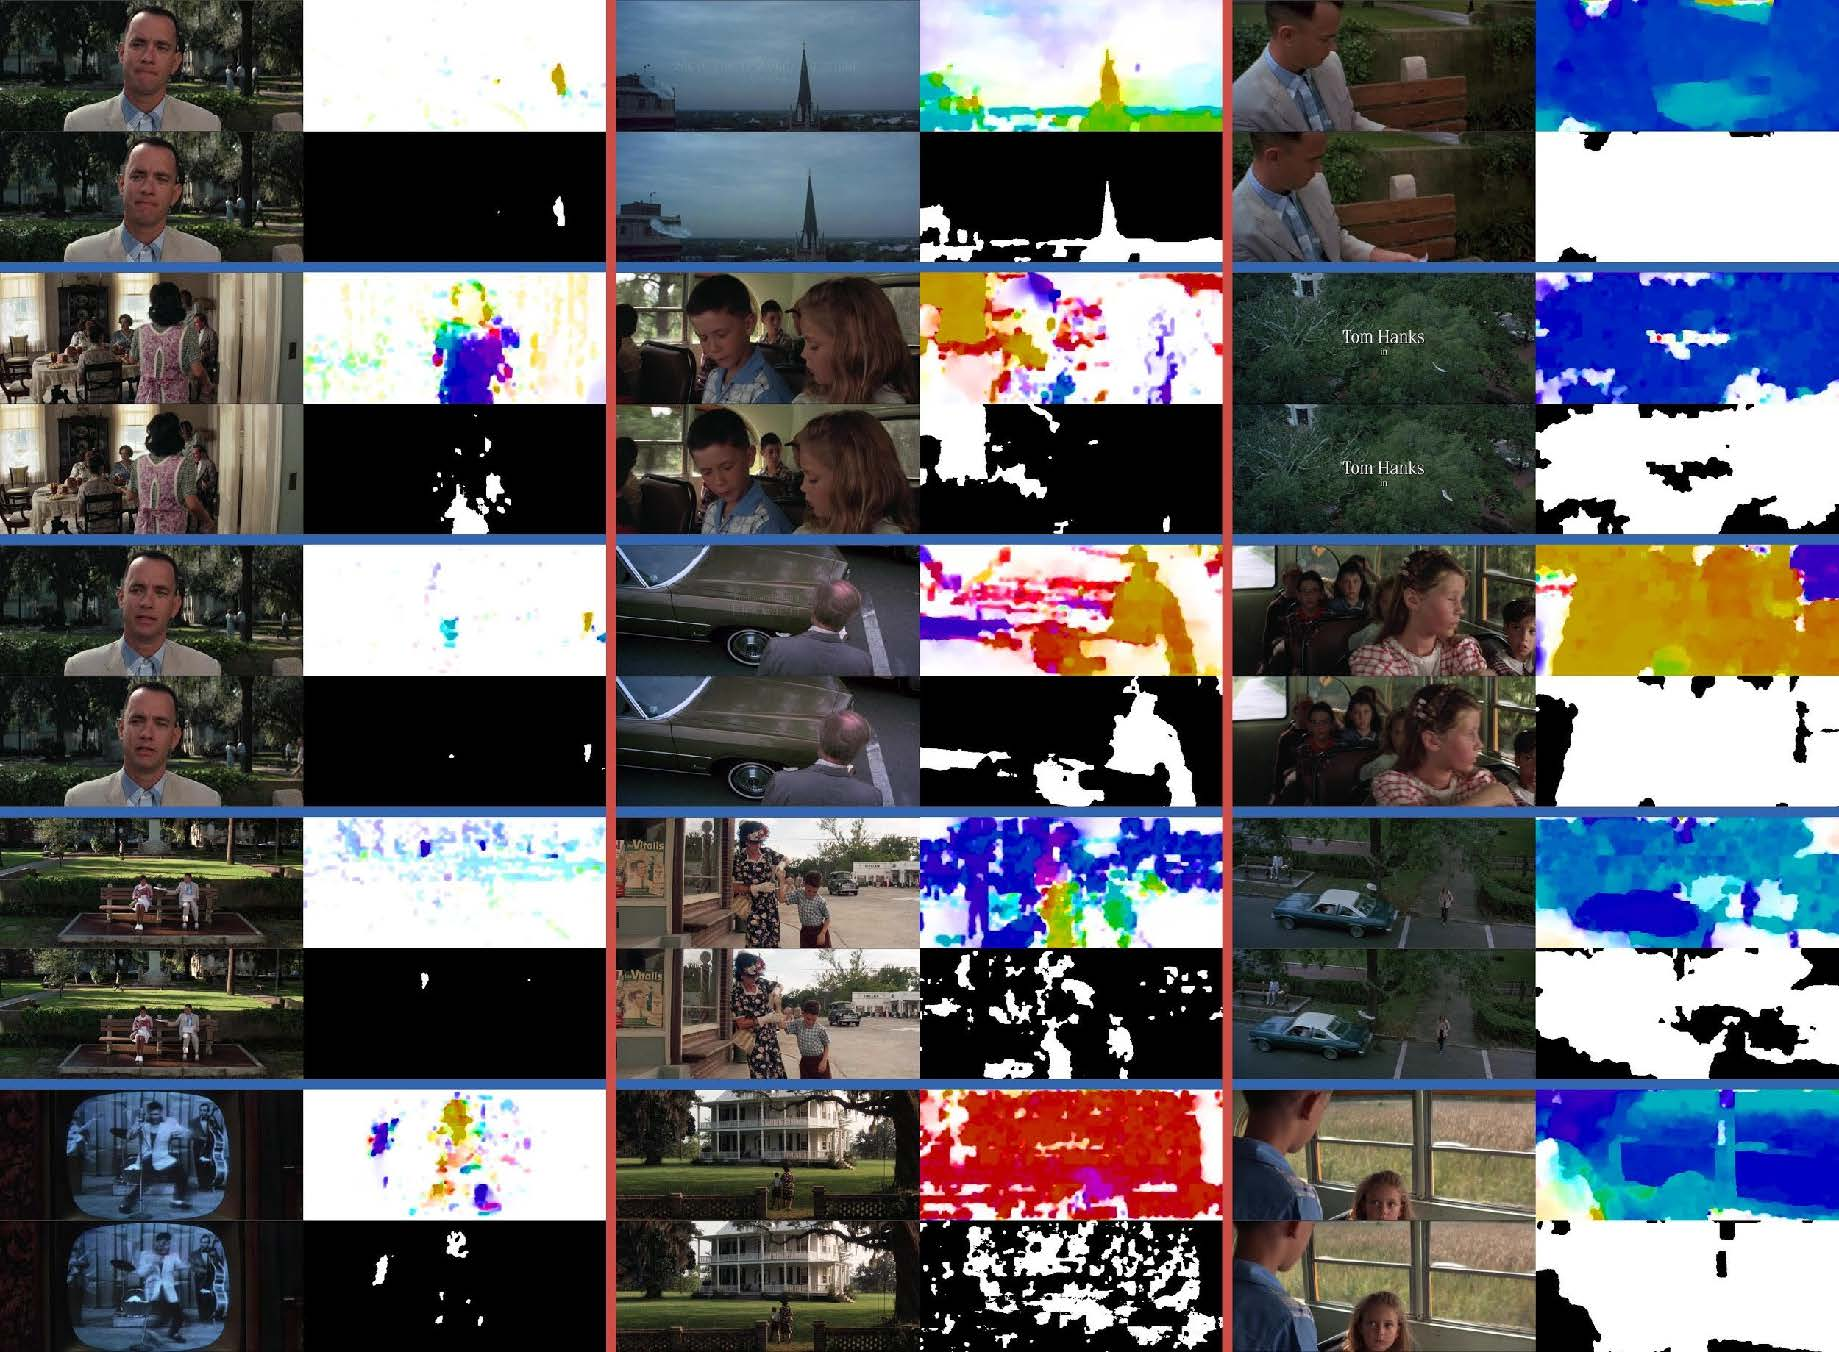
\includegraphics[width=6in]{./figures/C2Fig/motion_content.jpg}
%	\vspace{0.2em}
%	\caption{
%	15个样例帧和他们对应运动内容的可视化。
%	三个主要列中的每一个(使用红线分隔)表示帧运动的不同层次(低、中、高)。
%	在每个超级单元中,我们随机显示所选取的帧(左上),电影进度5帧之后的帧(左下),随机帧的光流(右上)、绝对运动门限为2像素的光流(右下)。
%	} 
%	\label{fig:motion_content}
%\end{figure*}


% k_E表示体素的数目
%\vspace{0.6em}
%\begin{figure*}[ht]
%	\centering
%	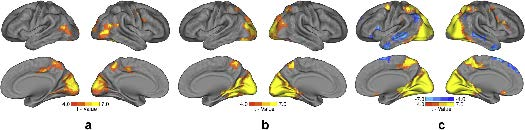
\includegraphics[width=1.0\textwidth]{./figures/C2Fig/BOLD_mean_responses.jpg}
%	\vspace{0.2em}
%	\caption{
%	当运动加入模型中,平滑跟踪和眼跳的平均效果,以及运动本身的平均效果(使用$P_{FWE}\textless0.05$,$P\textless0.001$的初始门限。
%	(a)与平滑跟踪相关的横跨两侧视觉脑区的激活($k_E=3706$,包括MT+/V5),以及两侧中扣带皮层延伸至楔前叶($k_E=605$)。
%	(b)与眼跳相关的两侧上延伸至楔前叶的激活($k_E=7715$)。
%	(c)运动相关的横跨两侧视觉脑区(包括MT/V5)和向上延伸至中扣带皮层和楔前叶的激活($k_E=10876$)。
%	同时也存在负激活,包括颞上沟皮层内侧(左:$k_E=450$;右:$k_E=456$)、颞顶联合区(左:$k_E=242$,右:$k_E=118$)和辅助运动区($k_E=304$)的两侧。
%	} 
%	\label{fig:BOLD_mean_responses}
%\end{figure*}


%\vspace{0.6em}
%\begin{figure*}[ht]
%	\centering
%	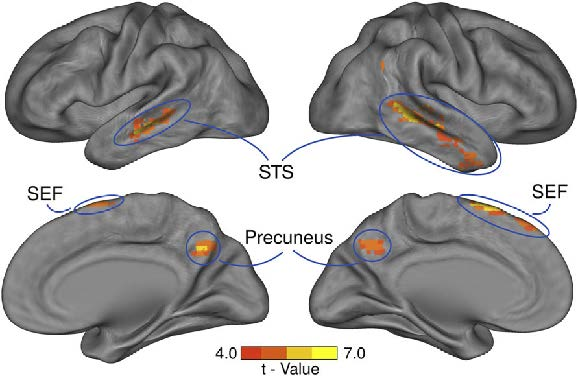
\includegraphics[width=1.0\textwidth]{./figures/C2Fig/SP_motion_contrast.jpg}
%	\vspace{0.2em}
%	\caption{
%	平滑跟踪大于运动和EpicFlow计算得到的运动回归变量对比的激活($p_{FWE}\textless0.05$,0.001的初始门限值)。
%	激活出现在右上/中颞回(前/后颞上沟)($k_E=536$,峰值xyz:60,-55,26)、左中颞沟(后 颞上沟)($k_E=194,峰值xyz:-60,-28,11$)、双侧楔前叶($k_E=102$,峰值xyz:6,-58,35)、双侧辅助视区($k_E=177$,峰值xyz:-6,11,62)。
%	} 
%	\label{fig:SP_motion_contrast}
%\end{figure*}


\subsubsection{结果鲁棒性} \label{sec:result_robustness}
当对某些数据进行模型拟合时,就像在 fMRI 中使用广义线性模型一样,想知道呈现的结果是否是所提供数据的唯一拟合或它们是否符合基础模式。
在这里,通过运行概念验证步骤(类似于 $k = 2$ 的 $k$ 重交叉验证)来评估呈现结果的鲁棒性。
首先将 8 个《阿甘正传》视频片段分成两半,前半部分包含视频段 1 到 4,下半部分包含视频段 5 到 8。
然后对广义线性模型进行拟合,该模型包括两个集合上各自的平滑跟踪回归变量和眼跳回归变量,并比较体素值以获取每个回归变量的平均效果。 
%图\ref{fig:fit_independently}中的
结果表明,两个模型的结果高度相关,线性拟合的 $r_2$ 为 0.81。




\subsection{核磁共振眼动分析}
这个实验分析的目的是分析在动态开放自然场景中与平滑跟踪相关的脑部激活。
为了这个目的,当动态场景作为刺激时,基于现成的算法和建模技术提出方法处理运动的噪声、非结构化的信息、以及来自扫描仪记录的眼跟踪数据。
这里主要的结果和之前的研究一致,当对平滑跟踪进行建模,显示在平滑跟踪时 MT/MST 有明显的激活。
当另外表示刺激运动内容的回归变量添加到模型当中,识别出了与注意力相关的区域,然而由于受血氧水平依赖平均效应诱发的类似平滑跟踪和运动,一些其他脑区(包括 MT/MST)降低到重要门限值以下。
%这些结果表明我们方法在简单交叉验证步骤中更加鲁棒(如图\ref{fig:fit_independently}所示)。


%\vspace{0.6em}
%\begin{figure*}[ht]
%	\centering
%	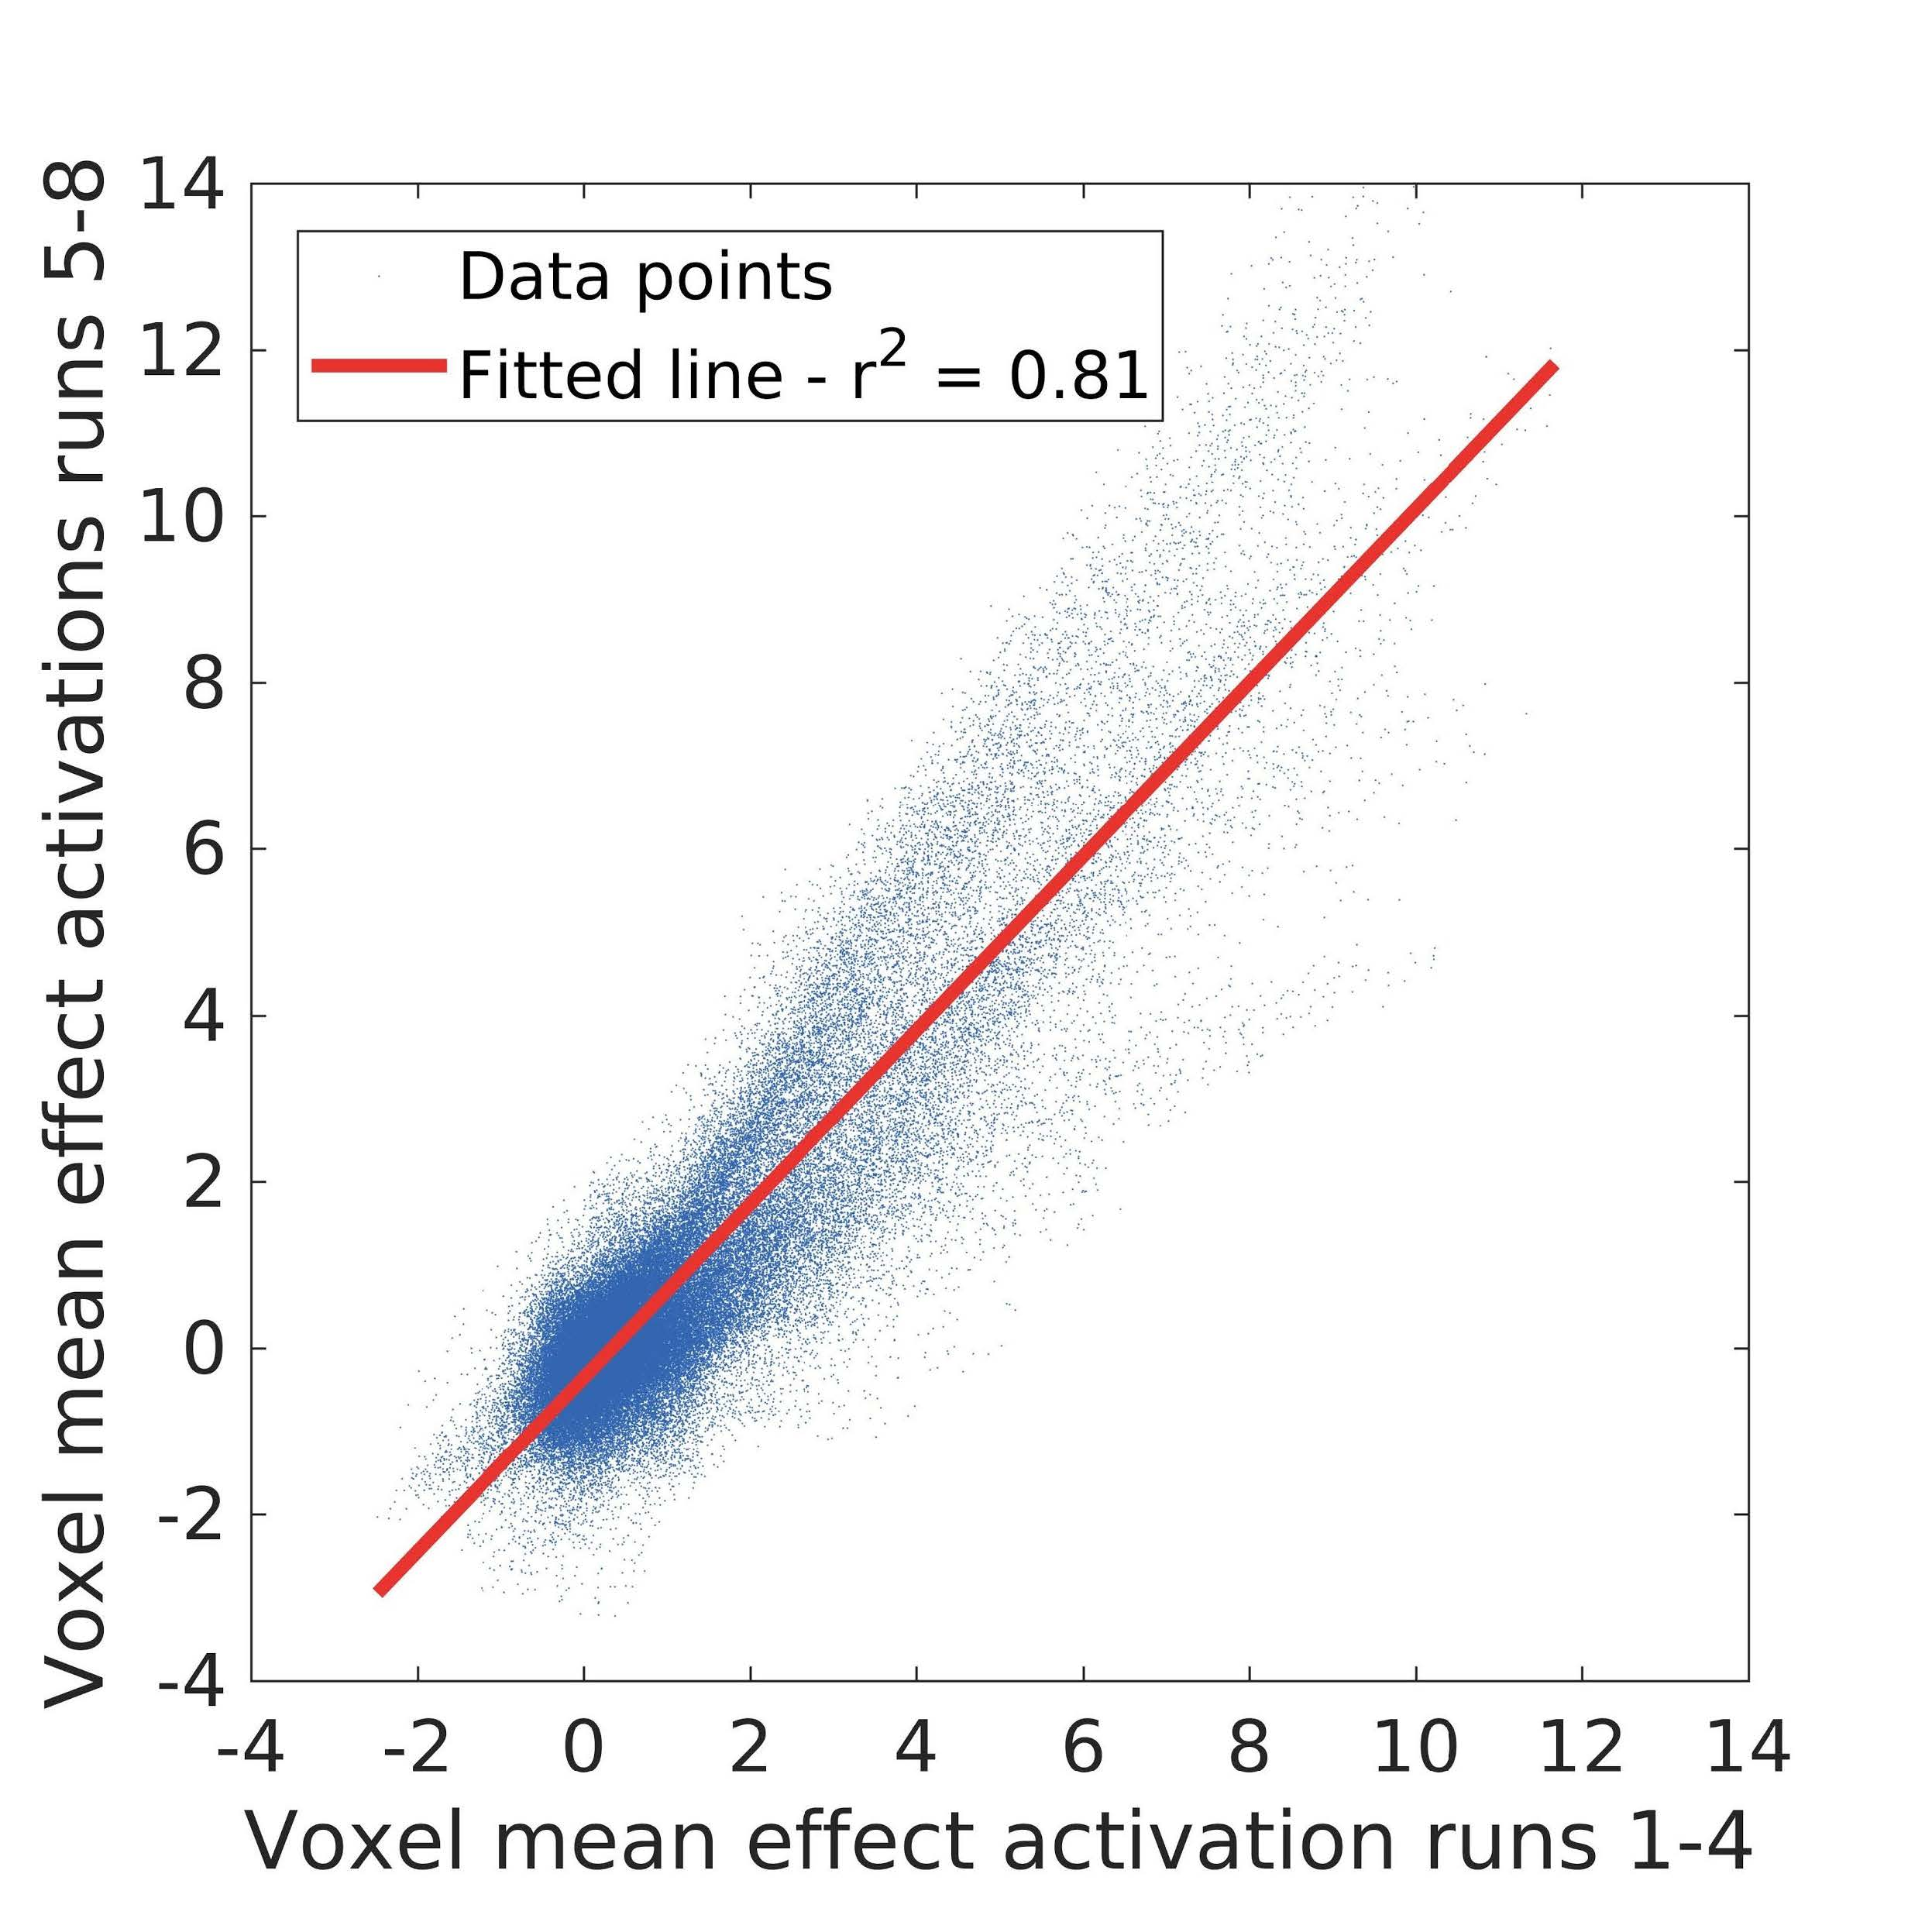
\includegraphics[width=1.0\textwidth]{./figures/C2Fig/fit_independently.jpg}
%	\vspace{0.2em}
%	\caption{
%	对于两个GLM模型,眼跳和平滑跟踪平均效果的体素激活是对于“StudyForrest”数据集的前半部分和后半部分独立拟合。
%	两个模型的体素值高度相关($r_2=0.81$),这表明我们的原始模型可以可靠地拟合数据。
%	} 
%	\label{fig:fit_independently}
%\end{figure*}




\subsubsection{模型中考虑运动的优势}
将运动作为回归变量添加到模型中,使得能够确定与平滑跟踪相关的激活,这些激活本身并非由刺激的整体运动所驱动
%(图\ref{fig:BOLD_mean_responses}a)。 
有趣的是,运动本身还会导致与颞上沟和辅助视区相关的负面激活。 
因此,当直接对比平滑跟踪大于运动时,这两个区域以及楔前叶在平滑跟踪期间的激活明显强于单独的运动内容。
%(图\ref{fig:SP_motion_contrast})。
颞上沟被认为是信息处理的枢纽,包括生物运动的处理~\cite{pinar2007superior,jastorff2009human,grossman2010fmr}以及需要社交认知的情况下的面部处理~\cite{allison2000social,hoffman2000distinct,lahnakoski2012naturalistic}。 
与该模型一致,通过经颅磁刺激抑制颞上沟活性导致难以感知生物运动~\cite{grossman2010fmr}。
此外,颞上沟活动的减少~\cite{freitag2008perception,alaerts2014underconnectivity} 与难以理解自闭症谱系障碍患者的生物运动和情绪内容有关~\cite{hubert2007brief,nackaerts2012recognizing,alaerts2014underconnectivity}。 
即使在目标不可见的情况下,辅助视区的激活也与预期的眼动相关,反映出认知输入可以独立于视觉输入而进行平滑跟踪规划~\cite{lencer2004cortical,missal2004supplementary,ohlendorf2010visual}。

在解释与运动内容有关的发现时,应考虑到运动回归变量是基于像素级运动能量的低层次描述,这可能无法捕获自然场景的语义特性。 
因此,根据分析,运动内容的高价值与背景和摄像机运动有关,这两者都广泛用于专业拍摄的电影视频中~\cite{cutting2011quicker}。
%,请参见图\ref{fig:motion_content}。
相反,将中等大小目标(比如具有社会意义的目标)的移动与低运动内容价值相关联。 
因此,除非执行对有意义目标的平滑跟踪,否则由运动内容回归变量建模的无关运动可能导致观察到的双向颞上沟和辅助视区中的负激活。


% 视频只要有运动的目标产生的脑激活
\subsubsection{视频中运动的解释}
为了从运动内容的相关脑激活中识别出平滑跟踪,在第一阶段个体层次分析中添加了一个额外的运动回归变量,它和眼动调制处理过程类似,再次将其建模为时间序列。
%这里使用 EpicFlow 算法显示结果,完整的帧表示运动建模(对于基于结构张量的较小值,该算法的结果定性上是相似的,数据这里没有显示)。
%为了更好的理解EpicFlow运动估计和我们运动回归变量之间的关系,参见图\ref{fig:motion_content}。
得到的运动回归变量和眼跳回归变量没有关系(皮尔逊相关系数 $r=-0.11$),并且对于平滑跟踪回归变量仍然有效(皮尔逊相关系数 $r=0.18$)。
%和平滑跟踪、眼跳、运动相关的血氧水平依赖响应的平均效果显示在图\ref{fig:BOLD_mean_responses}中。
%从图\ref{fig:BOLD_mean_responses}a和b中可以看出,平滑跟踪和眼跳激活与图\ref{fig:sp_sac_activation}中在定量上非常接近,但是当运动加入模型(图\ref{fig:BOLD_mean_responses}a)中时,平滑跟踪有更小的大小和强度。
%平滑跟踪相关激活的减少伴随着强烈的运动(图\ref{fig:BOLD_mean_responses}c)相关激活(大致和平稳跟踪有相同的激活区域,如图\ref{fig:sp_sac_activation}a所示)。
然而,颞上沟皮层内层的激活和辅助眼区的辅助运动皮层与运动回归变量是负相关。

按照这个模型,平滑跟踪大于眼跳的对比仅仅在中扣带皮层和右侧颞顶联合区区域产生重要的激活。
%图\ref{fig:contrast}a中,
MT/MST 和楔前叶的激活没有达到 $p_{FWE} < 0.05$ 的要求门限。
%
平滑跟踪大于运动的对比揭示了在颞上沟皮层内层、楔前叶和辅助视区的辅助运动区的双侧激活。
与之相反,眼跳大于运动的对比没有揭示任何重要的激活区域。

\subsubsection{额外回归变量的考虑}
为了至少部分缓解运动能量分析的潜在混乱,引入了建模基本视频特征的其他回归变量。 
在两个控制实验中,将基于显著性和边缘密度的场景动态开放性的建模,作为吸引注意力的参数,以测试这些参数是否干扰了与平滑跟踪和运动内容有关的激活。
在这两种情况下,验证回归变量的平均效果均显示出在一些非常小的簇中的重要激活(在大脑后部总体上大约为 150-300 个体素,大部分在视觉皮层中),但并未影响涉及兴趣主要对比的激活。 
根据这些观察结果得出结论,根据对每个特征建模的方式,眼动规划过程主要受基础运动的驱动。 
但是,在将来对动态自然场景中平滑跟踪的研究中,可能需要对所有潜在参数和建模技术进行更详尽的搜索。


\subsubsection{平滑跟踪中与变化相关的脑区}
平滑跟踪大于眼跳与仅在第一层次设计矩阵中包括的平滑跟踪和眼跳回归变量的对比,揭示了中扣带皮层和楔前叶的激活,这先前与平滑跟踪眼动控制~\cite{tanabe2002brain,kimmig2008fmri}和视觉空间处理有关~\cite{berman1999cortical,e2006the}。
此外,与右颞顶联合区相关的眼跳相比,这种对比在平滑跟踪期间产生了更高的激活度,而右颞顶联合区是涉及向未注意区域提供指导的区域~\cite{corbetta2000voluntary,wu2015a,marsman2016a}。
最重要的是,这种对比揭示了与 MT/MST 区域相关的双边激活,该区域被视为核心运动处理区域~\cite{petit1999functional,lencer2008neurophysiology,nagel2006parametric},并且在以前的研究中与平滑跟踪眼动有关~\cite{kimmig2008fmri,ohlendorf2010visual,marsman2016a}。 
值得注意的是,当添加第三回归变量建模的整体刺激运动时,MT/MST 区域变得不那么显著。 
最好的解释是,这一区域的血氧水平依赖响应方差现在由两个回归变量(平滑跟踪和运动)而不是一个回归变量共享~\cite{ohlendorf2010visual},
%,这从图\ref{fig:BOLD_mean_responses}a和c中的平滑跟踪和运动的平均效果可以看出。 
这证明了在动态开放场景中找到单一激活源很困难,许多不同的因素可能会激发特定区域的激活,而这种混淆的完全解开可能难以做到。

%\subsubsection{平滑跟踪相关激活}
%\subsubsection{平滑跟踪和眼跳的对比激活}
% saccade 眼跳
经过组织和分析,平滑跟踪作为所感兴趣的眼动,识别出和眼跳相关的三个脑区。
%因此,我们关心的是在观看自然场景时平滑跟踪和眼跳相关脑区的不同之处。
%当$P_{FWE}\textless0.05$和$P\textless0.001$的初始门限值时的对比在图\ref{fig:contrast}中进行可视化。
%在图\ref{fig:contrast}a中,
第一个脑区有运动处理和平滑跟踪相关脑区 MT/MST 的双边激活(左),第二个脑区包括中扣带皮层并延伸至楔前叶,第三个脑区包括右颞顶联合处的一个激活。
%图\ref{fig:contrast}b展示了
%眼跳大于平滑跟踪的对比在 V2 有重要的激活响应(右:$k_E=91$)。
%平滑跟踪和眼跳相关的血氧水平依赖响应的平均效果如图\ref{fig:sp_sac_activation}表示,
这里使用 $p\textless0.001$ 的初始门限在 $p_{FWE}\textless0.05$ 时进行聚类。
该过程共产生三个和平滑跟踪相关的聚类。
%和两个和眼跳相关的聚类(Sac1 到 Sac2)。
%参见表\ref{tab:clusters}。
% Sac1相比于SP1颞中回有多一块橙色小区域
第一个区域最明显的是在中颞回内的最大激活,推测可能是因为 该区域包含视觉运动区域 MT/MST,这在意料之中,因为这些区域和平滑跟踪和运动处理都有关。
第二个大的聚类主要覆盖中扣带皮层和楔前叶的部分区域。
% (a)中右图为右脑,rTPJ和注意力和社会认知相关。
%同时这里也存在一个更小的和眼跳相关的聚类 Sac2,他覆盖了楔前叶的部分区域,
第三个和平滑跟踪相关的一个更小的聚类是右侧颞顶联合区。
为了检查显示的每个眼动聚类都很好的表示了对应脑区,使用了一个简单的交叉验证步骤(详细过程参考章节~\ref{sec:result_robustness})。
%两个独立模型激活之间的高度相关性($r^2=0.81$)表明回归模型不仅仅提供了数据,而且拟合了一种模式。



%表\ref{tab:anat_func_area}列出了更加详细的解剖和功能区域的描述,分别包括识别出的聚类SP1-SP3和Sac1-Sac2。
%解剖区域使用自动解剖地图集进行分割\cite{tzourio-mazoyer2002automated,rolls2015implementation}。
%为了避免相对较少体素的解剖区域弄乱表格,我们用聚类中体素数目百分比作为裁剪门限值。
%对于两个最大表中两个最大聚类的门限值设置为$-2\%$,其他的设置为$5\%$。


%\begin{figure*}[ht]
%	\centering
%	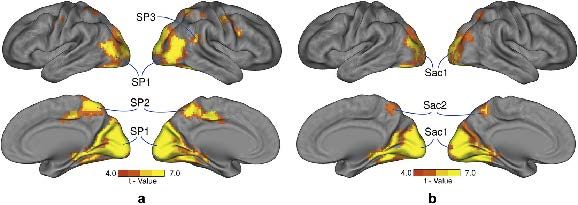
\includegraphics[width=6in]{./figures/C2Fig/sp_sac_activation.jpg}
%	\vspace{0.2em}
%	\caption{平滑跟踪和眼跳相关的激活。
%		(a)平滑跟踪相关的激活(使用$p_{FWE}<0.05$,$p<0.001$的初始化门限。
%		激活横跨大脑两边的视觉区域(SP1:$k_E=7647$,包括与平滑跟踪相关的MT+/V5),
%		(脑两边的)中扣带皮层延伸到楔前叶(后顶叶皮层的一部分,位于头顶叶内侧部分)(SP2:$k_E$=2048),
%		右颞顶连接处(SP3:$k_E=109$)。
%		(b)眼跳相关的激活(使用$p_{FWE}<0.05$,$p<0.001$的初始门限值。
%		激活横跨两边大脑的视觉区域(Sac1:$k_E=6437$)和楔前叶(Sac2:$k_E=245$)。
%		分区的详细列表参考表。
%	} 
%	\label{fig:sp_sac_activation}
%\end{figure*}


%\vspace{0.6em}
%\begin{table}[htbp]\wuhao
%	\centering
%	\caption{和平滑跟踪和眼跳眼动相关,带峰值激活T值的聚类列表和沿着聚类层次FWE校正p值的定位。
%		}
%	\vspace{0.3em}
%	\begin{tabular}{p{1.7cm}<{\centering}p{1.7cm}<{\centering}p{1.7cm}<{\centering}p{1.7cm}<{\centering}p{1.7cm}<{\centering}p{1.7cm}<{\centering}p{1.7cm}<{\centering}}
%		\toprule[1.5pt]
%		聚类名字  & X  & Y   & Z & 聚类大小 &$P_{FWE_corr}$ &t峰值\\ 
%		\midrule[1.0pt]
%		SP1     &-3 &-91 &14 &7647 &\textless0.001  &15.11 \\
%		SP2   &6 &-43 &56 &2048  &\textless0.001  &8.48  \\
%		SP3   &57 &-40 &17 &109  &0.011  &6.94  \\
%		Sac1   &-9 &-82 &17 &6437  &\textless0.001  &16.84  \\
%		Sac2   &-6 &-52 &56 &245  &\textless0.001  &6.25  \\
%		\bottomrule[1.5pt]
%	\end{tabular}
%	\label{tab:clusters}
%\end{table}


%\vspace{0.6em}
%\begin{table}[htbp]\wuhao
%	\centering
%	\caption{涉及平滑跟踪和眼跳相关聚类(着以灰色)的脑区列表,只与平滑跟踪有关标成白色。
%	可视化门限值对于大聚类选择表\ref{tab:clusters}的$2\%$,对于小聚类选择$5\%$。
%	因此在每个聚类中这些值的总和不等于体素的总数。
%	}
%	\vspace{0.3em}
%	\begin{tabular}{p{1.2cm}<{\centering}|p{1.2cm}<{\centering}|p{0.5cm}<{\centering}|p{0.5cm}<{\centering}|p{0.5cm}<{\centering}|p{1.0cm}<{\centering}|p{1.0cm}<{\centering}|p{1.0cm}<{\centering}|p{0.5cm}<{\centering}|p{0.5cm}<{\centering}|p{0.5cm}<{\centering}|p{0.5cm}<{\centering}|p{0.5cm}<{\centering}|p{0.5cm}<{\centering}}
%		\toprule[1.5pt]
%		解剖区域  & 功能区域(布罗德曼分区)  & X   & Y & Z &所属 &体素数 &T峰值 &X &Y &Z &所属 &体素数 &T峰值 \\ 
%		\midrule[1.0pt]
%		左舌回     &17,18 &-15 &-76 &2 &SP1  &528 &12.04 &-18 &-79 &2 &Sac1 &522 &14.00 \\
%		\midrule[1.0pt]
%		右舌回     &17,18 &-12 &-85 &13 &SP1  &528 &12.04 &-18 &-79 &2 &Sac1 &522 &14.00 \\
%		\midrule[1.0pt]
%		左距状皮层     &17,18,30 &-12 &-85 &13 &SP1  &528 &12.04 &-18 &-79 &2 &Sac1 &522 &14.00 \\
%		\midrule[1.0pt]
%		右距状皮层     &17,18,30 &-12 &-85 &13 &SP1  &528 &12.04 &-18 &-79 &2 &Sac1 &522 &14.00 \\
%		\midrule[1.0pt]
%		左楔叶     &18,19 &-12 &-85 &13 &SP1  &528 &12.04 &-18 &-79 &2 &Sac1 &522 &14.00 \\
%		\midrule[1.0pt]
%		右楔叶     &18,19 &-12 &-85 &13 &SP1  &528 &12.04 &-18 &-79 &2 &Sac1 &522 &14.00 \\
%		\midrule[1.0pt]
%		左枕上     &18,19 &-12 &-85 &13 &SP1  &528 &12.04 &-18 &-79 &2 &Sac1 &522 &14.00 \\
%		\midrule[1.0pt]
%		右枕上     &18,19 &-12 &-85 &13 &SP1  &528 &12.04 &-18 &-79 &2 &Sac1 &522 &14.00 \\
%		\midrule[1.0pt]
%		左枕中     &19,37(V5) &-12 &-85 &13 &SP1  &528 &12.04 &-18 &-79 &2 &Sac1 &522 &14.00 \\
%		\midrule[1.0pt]
%		右枕中     &19,37 &-12 &-85 &13 &SP1  &528 &12.04 &-18 &-79 &2 &Sac1 &522 &14.00 \\
%		\midrule[1.0pt]
%		左枕下     &18 &-12 &-85 &13 &SP1  &528 &12.04 &-18 &-79 &2 &Sac1 &522 &14.00 \\
%		\midrule[1.0pt]
%		左梭状回     &18,19 &-12 &-85 &13 &SP1  &528 &12.04 &-18 &-79 &2 &Sac1 &522 &14.00 \\
%		\midrule[1.0pt]
%		右梭状回     &18,19 &-12 &-85 &13 &SP1  &528 &12.04 &-18 &-79 &2 &Sac1 &522 &14.00 \\
%		\midrule[1.0pt]
%		左小脑 6     &- &-12 &-85 &13 &SP1  &528 &12.04 &-18 &-79 &2 &Sac1 &522 &14.00 \\
%		\midrule[1.0pt]
%		右小脑 6     &- &-12 &-85 &13 &SP1  &528 &12.04 &-18 &-79 &2 &Sac1 &522 &14.00 \\
%		\midrule[1.0pt]
%		左楔前叶     &5,7 &-12 &-85 &13 &SP1  &528 &12.04 &-18 &-79 &2 &Sac1 &522 &14.00 \\
%		\midrule[1.0pt]
%		右楔前叶     &5,7 &-12 &-85 &13 &SP1  &528 &12.04 &-18 &-79 &2 &Sac1 &522 &14.00 \\
%		\midrule[1.0pt]
%		左中颞     &19,39(V5) &-12 &-85 &13 &SP1  &528 &12.04 &-18 &-79 &2 &Sac1 &522 &14.00 \\
%		\midrule[1.0pt]
%		右中颞     &19,39(V5) &-12 &-85 &13 &SP1  &528 &12.04 &-18 &-79 &2 &Sac1 &522 &14.00 \\
%		\midrule[1.0pt]
%		右下颞     &37(V5) &-12 &-85 &13 &SP1  &528 &12.04 &-18 &-79 &2 &Sac1 &522 &14.00 \\
%		\midrule[1.0pt]
%		左中扣带皮层     &23,24,31 &-12 &-85 &13 &SP1  &528 &12.04 &-18 &-79 &2 &Sac1 &522 &14.00 \\
%		\midrule[1.0pt]
%		右中扣带皮层     &23,24,31 &-12 &-85 &13 &SP1  &528 &12.04 &-18 &-79 &2 &Sac1 &522 &14.00 \\
%		\midrule[1.0pt]
%		旁中央小叶     &5 &-12 &-85 &13 &SP1  &528 &12.04 &-18 &-79 &2 &Sac1 &522 &14.00 \\
%		\midrule[1.0pt]
%		右上颞     &40 &-12 &-85 &13 &SP1  &528 &12.04 &-18 &-79 &2 &Sac1 &522 &14.00 \\
%		\midrule[1.0pt]
%		右上缘回     &40 &-12 &-85 &13 &SP1  &528 &12.04 &-18 &-79 &2 &Sac1 &522 &14.00 \\
%		\bottomrule[1.5pt]
%	\end{tabular}
%	\label{tab:anat_func_area}
%\end{table}



%完整的解剖区域列表是这些聚类的一部分,在表\ref{tab:anat_func_area}中提供。


%\begin{figure*}[ht]
%	\centering
%	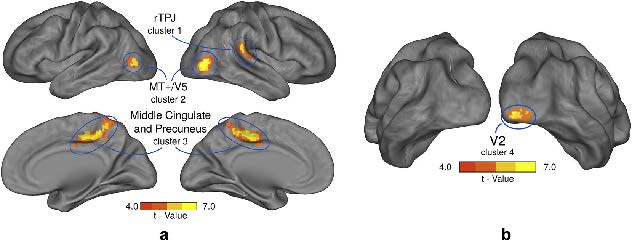
\includegraphics[width=6in]{./figures/C2Fig/contrast.jpg}
%	\vspace{0.2em}
%	\caption{
%	(a)使用0.001的初始化门限值,在$P_{FWE}\textless0.05$时,平滑跟踪大于眼跳的激活状态。
%	两侧MT/V5处的激活(右边:$k_E=169$,左边$k_E=89$),中扣带皮层延伸至楔前叶($k_E=665$),右颞顶联合区(rTPJ)($k_E=158$)。
%	(2)在0.001的初始门限且$p_{FWE}\textgreater0.05$时眼跳大于平滑跟踪的激活。
%	V2处的激活(右:$k_{E}=91$)。
%	} 
%	\label{fig:contrast}
%\end{figure*}








%\subsubsection{自然观看条件下缺乏前额叶视区的关联}
%我们没有检测到任何和前额叶视区相关的激活,该区域涉及到平滑跟踪和眼跳的规划和执行~\cite{sp_representation,berman1999cortical,gagnon2006transcranial,kimmig2008fmri}。
%一个可能的解释是在典型的实验中,受试在长久注视基线周期和点跟踪或者场景观察之间进行切换。
%相反,在我们这里使用的数据集中,受试在连续观察电影时,可能从事一些眼睛运动的规划,这对真实世界观察行为更具有代表性。
%因此,这些变化(比如在连续2秒时间窗口的眼跳)不足以识别出所有眼跳相关的激活(包括FEF)。
%另一个限制因素可能是FEF太小,在特定实验条件和操作中报告依靠激活的位置有较大的方差。
% 被平均了?


\subsection{类脑跟踪模型的有效性}
在这里比较了各种实验结果,以解释为什么所提出的 BTN 是一个类脑跟踪模型。
很容易看出,模型架构和训练过程与现有的视觉跟踪模型实现略有不同。
%
图~\ref{fig:neural_predictivity}(a)展示了进行激活对比的区域为 BTN 的动态滤波网络和大脑皮层的中颞和上颞内侧区;
图~\ref{fig:neural_predictivity}(b)展示了 BTN 在 Tracking-Gump 数据集上 BTS 的性能,获得了最好 0.365 的类脑跟踪分数。
并且获得最高跟踪分数的模型在 Tracking-Gump 数据集上也有出色的类脑跟踪分数,
表明 Tracking-Gump 数据集上的跟踪效果和皮层激活模式之间存在联系。
如图所示~\ref{fig:neural_predictivity},表明具有良好 Tracking-Gump 跟踪性能的模型与 BTS 具有很强的相关性,并且在 Tracking-Gump 数据集中存在显著的相关性($p \textless 0.05$)。
% todo

% 纵坐标:神经预测性、分数 的归一化值
%\begin{figure}[t]
%	\centering
%	\includegraphics[width=0.75\linewidth]{figures/C2Fig/comp_sim.pdf}
%	\caption{
%		BTN 捕获的 MT/MST 神经响应
%	}
%	\label{fig:neural_predictivity}
%\end{figure}

\begin{figure}[htbp]
	\centering
	
	\subfigure[BTN 和大脑进行激活对比的区域]{
		\begin{minipage}[t]{0.35\linewidth}
			\centering
			\includegraphics[width=1\textwidth]{./figures/C2Fig/similarity.pdf}
		\end{minipage}%
	}%
	\subfigure[BTN 捕获的中颞和上颞内侧区神经响应]{
		\begin{minipage}[t]{0.65\linewidth}
			\centering
			\includegraphics[width=1\textwidth]{./figures/C2Fig/comp_sim.pdf}
		\end{minipage}%
	}%
	%\n is important,(or \quad) 

	
	\centering
	\caption{BTN 与大脑激活响应的对比}
	\label{fig:neural_predictivity}
\end{figure}


% 改变跟踪模型参数(模型的深度)来看效果
% 换其他的单目标跟踪模型(IoU;激活相似性?)
% 紧致性+循环性验证
\subsubsection{BTN 与大脑皮层的结构相似性}
该研究设计了一个类脑跟踪神经网络 BTN,它比经典深度神经网络更紧密地遵循神经解剖学对齐。
此外,根据 BTS 在 Tracking-Gump 数据集上的测试性能,BTN 实现了良好的视觉跟踪性能。
因此,BTN 既满足神经科学中的神经解剖学限制,又能很好地满足计算机视觉中的工程要求。

因为 BTN 限制了模块的数量并使用了循环结构,实验发现 BTN 比当前优秀的深度神经网络跟踪模型更接近神经解剖学约束。
在神经科学中,因为没有神经学上可信的训练方法,用于训练平滑跟踪的类脑深度神经网络,它可以使用更好的神经解剖学和连接机制。
例如,使用跨层链接~\cite{he2016deep} 解决深度神经网络训练过程中梯度消失的问题并非是受大脑机制启发。
如图~\ref{fig:structure_analysis} 所示,考虑到各种网络架构,在找到合适的类脑架构 BTN 之前测试了各种架构配置。
实验分析了四个主要因素,包括 $\rm{CONV_{V1}}$ 中的初始步长、$\rm{DFN_{MT/MST}}$ 中的动态滤波器的数目、$\rm{LSTM_{FEF}}$ 和 $\rm{FC}$ 中隐藏单元的数量。
每行表示当某个超参数发生变化时,皮层相似性分数和行为相似性分数如何根据训练的 BTN 变化。

% 证明能够捕获时间序列上的信息
% 神经相似性分数 的图
\subsubsection{BTN 捕获的 MT/MST 神经响应}
\label{sec:capture_neural}

前馈神经网络无法预测时间序列的趋势,因此无法捕获跟踪模型的类脑响应~\cite{kar2019evidence, TangSchrimpfLotter2018Recurrent}。
通过使用循环连接,BTN 能够预测相应皮层中随时间变化的激活。
最新研究工作~\cite{kar2019evidence} 发现图像分类中的可解码结果是在颞下皮层神经元中产生的,
并且这些输入对于深度神经网络来说很难在颞下区域花费更多时间进行解码。
时间属性激发了一个类脑网络的假设:
它是否会随着时间的推移预测 MT/MST 皮层激活中的逐帧运动信息?
因此,当有明显的目标运动特征可用时,BTN 能够预测视频帧中的运动,
并将其与人类 MT/MST 皮层中记录的反应进行比较。
值得注意的是,BTN 从未学会预测人类皮层的响应强度。
但是却学习到了可以解码神经响应和模型响应之间的运动相似性特征。
当使用 PCA 方法进行数据压缩时,更多的组件将保留更多的神经信息。
如图~\ref{fig:neural_predictivity} 所示,最后评估了 BTN 在人类大脑皮层的 MT/MST 中捕获到了细粒度运动响应的能力,
%并给出了 0.365 ($p < 0.05$) 的 BTS。
显示了对于不同 PCA 分量所表现出的归一化神经相似性和 $p$ 值。
当 PCA 组件的数量达到 90 时,BTN 的神经预测性获得了最佳 0.365 的结果。


\subsubsection{Tracking-Gump 数据集上 BTN 的有效性}
跟踪性能在后期训练中确实提高了皮层相似度,在一系列模型中选择了具有最大 BTS 的模型。
此外,模型预测的边界框与眼睛注视的位置大致一致。
最后,在实验中使用行为和 MT/MST 相似性指标来分析 BTN 中的运动信息。
BTN 在 Tracking-Gump 数据集上实现了出色的跟踪性能,如图~\ref{fig:tracking} 所示,
对于不同的视频序列,用边界框来标识模型的预测轨迹。
此外,这些受试的平均眼睛注视位置由圆进行标识,并且其面积与跟踪时人眼瞳孔大小成正比。
该实验证明了所提出的 BTN 在动态开放环境中的有效性和鲁棒性。

\begin{figure}[t]
	\centering
	\includegraphics[width=\linewidth]{figures/C2Fig/tracking.pdf}
	\caption{
		在 Tracking-Gump 数据集上测试所提出的类脑跟踪模型的效果示例	
	}
	\label{fig:tracking}
\end{figure}

\subsection{讨论}

在该研究工作中,设计了用于预测人脑平滑跟踪的类脑跟踪模型 BTN,实现了预测机制和在线跟踪随意运动的目标。
可以看出,BTN 利用深度神经网络实现神经解剖的对齐、人眼跟踪行为和大脑激活响应的预测,
并且实验结果表明 BTN 可以产生连续的预测跟踪信号。
尽管平滑追踪研究表明,物体运动的皮层表征可能被用于跟踪推理~\cite{b21,b4,b3},但建立和保持皮层表征的皮大脑层理论是未知的。
这项研究表明,通过 BTN 在线学习和更新皮层表示可以减少跟踪滞后,在面对漂移或遮挡时调整眼球运动并产生连续跟踪。

平滑跟踪的一个有趣特征是,当遮挡发生时跟踪运动会继续进行。
BTN 无延迟地跟踪运动物体时,视网膜有运动动作。
在学习了物体运动特征后,视网膜滑移很小。
然而,小的视网膜滑动不能进行被遮挡的对象跟踪,
LSTM 却可以产生自我维持的眼动预测~\cite{kashyap2018a},
小的视网膜滑动成分持续用于调整跟踪的预测。
当发生遮挡时,这种可调节的视网膜滑动信息不存在。
因此,就像之前的研究结果一样~\cite{b4},跟踪是一步一步丢失的。
此外在 BTN 中,LSTM 中的每个神经元都有基础的自发激活。
当被跟踪目标被遮挡时,训练好的激活模型会不断产生跟踪信号。

\subsubsection{损失函数分析}
之前的实验表明使用循环注意力跟踪器能够跟踪真实世界的的目标。
除了和循环注意力跟踪器~\cite{ratm} 相似的地方外,本章的方法还使用了额外的模块,包括:边界框回归损失、背侧流损失、腹侧流损失和辅助损失,并将这些损失组合在一个统一的方法中,
现在讨论这些模块的属性。

(1)背侧流中的空间注意力损失防止梯度消失:早期的实验表明仅仅使用跟踪损失会导致梯度消失问题。
在训练的初期,改模型不能正确地估计目标的运动,导致不能抽取跟踪目标的前景,或者仅仅包含跟踪目标的一部分。
这种情况下,监督信号和模型的输入没什么联系,阻止了学习的进行。
即使当目标包含在前景中,因为任何指导信号不得不通过特征抽取阶段传向之前时间步,导致损失函数回传的梯度路径相当长。
因此,直接惩罚注意力参数可以解决这个梯度消失的问题。

(2)空间注意力始终有效:
为了使跟踪系统适应目标的外观,并且和开始位置无关,实验中将初始的边界框转化为注意力参数,在这里增加了偏置值,并从对应的视觉特征创建 LSTM 的隐藏状态。
在实验中,偏置值始终收敛到正值,相比于目标的边界框更加偏向于注意力前景。
表明对于目标跟踪丢弃不相关的特征是可取的,基于注意力模块,整个跟踪系统在空间注意力和外观注意力权衡重要性。

(3)腹侧流中外观注意力是必要的:给足够多的数据和足够大的模型容量,外观注意力能够在更新工作记忆之前过滤掉不相关的输入特征。
然而,一般情况下,如果模型使用合适的损失进行限制会加快训练的过程。
%图中展示模型使用和不使用外观注意力情况下,提取前景和对应位置映射的例子。
使用外观注意力情况下,即使跟踪的行人被其他人遮挡也能跟踪上。
而没有惩罚时,目标定位可能不会非常好,甚至可能丢失整个目标。
通过使用外观注意力损失,不仅能提升跟踪的效果,而且使模型更加具有可解释性。




\subsubsection{MT/MST 和 FEF 在目标跟踪中的作用}
许多研究都发现 FEF 拥有预测目标跟踪的能力。
当物体被遮挡或出现时,FEF 的去除或损伤会损害猴子对运动物体的跟踪~\cite{b11}。
FEF 中的神经元激活表明,在移动目标消失后,连续激活仍密集地存在~\cite{b14}。
此外,一些 fMRI 工作发现在 FEF~\cite{b33} 中存在预测眼球跟踪的运动指标。
本研究工作表明,FEF 提取了对象运动模式的皮层表示来指示预测跟踪过程。

FEF 接收来自 MT/MST 的密集映射,这些映射是背流中处理移动目标的区域。
如图~\ref{fig:c2:introduction} 所示,在后半部分,FEF 的输出被传递到脑干区域的背侧 脑桥核,
此外,这些脑干区域将信号从 FEF 传递到脑桥核,从而进行眼部调整~\cite{b36}。

神经解剖消去的结果表明,FEF 从顶叶区域获得输入并输出到脑桥核以控制眼球运动~\cite{b11}。
这些结果表明 FEF 与 LSTM 具有可靠的皮层相关性,这是基于对象跟踪预测能力的。
此外,FEF(LSTM)使用图像刺激来推断眼球运动信号以进行眼动调整。

\subsubsection{BTN 的应用和局限性}
本研究所提出的 BTN 不仅可用于传统的视觉对象跟踪任务,
此外它还是是一种更具解释性的类脑跟踪模型,可用于预测眼睛注视的位置和皮层通路中的激活。

尽管如此,独立的训练配置可能是训练深度神经网络的基本特征~\cite{Kornblith2018a}。
此外,辅助任务对分数的影响不是很大,但显著提高了迁移效果~\cite{Kornblith2018a}。
因为 BTN 是一个迁移学习问题,所以不能排除在使用不同的训练设置时 BTS 可能会发生变化。
他们通过使用优化的配置重新训练深度学习网络可以极大地提高迁移效果~\cite{Kornblith2018a}。
因此,一般认为只有特定的训练 BTN 是最优的,而不是所有的网络架构模型。
实际上可以执行网格搜索以根据验证集的性能选择最佳训练配置。

\subsubsection{深度神经网络与神经科学的关系}

构建类脑架构模型 BTN 的一个重要步骤是类脑跟踪分数 BTS,它是将深度神经网络与目标跟踪时的大脑皮层进行比较的定量指标。
尽管到目前为止还没有皮层跟踪指标,但所提出的框架是一个有启发性的想法。
首先,所提出的框架扩展了探索性研究,表明跟踪性能与皮层相似性相关。
然而,循环结构的使用改变了这种趋势,并且与大脑皮层具有极好的神经解剖学相似性。
此外,发现 Tracking-Gump 跟踪分数与 BTN 中的 BTS 之间可能存在冲突。
视觉目标跟踪有很多优秀的模型,在 BTS 中没有较高的分数,这些没有较好 BTS 的深度学习模型却可能会在 Tracking-Gump 数据集上取得较好的跟踪效果。
此外,发现有些深度神经网络不仅具有出色的 BTS 性能,而且可以轻松获得良好的跟踪结果,这支持了 BTS 是一个综合指标的假设,并且这些结果不仅仅基于所使用的行为和神经数据集。


使用 BTS 的相似性量化来比较这些深度神经网络,
并评估 BTS 上各种行为和神经数据集的指标。
对于 BTN,实验证明了根据解剖对齐的和循环结构的皮层解剖模型可以通过皮层激活预测、逐帧行为甚至神经动力学很好地学习皮层机制。
这样,BTN 可以同时获得较高的 Tracking-Gump 跟踪性能和突出的类脑效果。
总的来说,该研究表明了类脑模型是深度学习和神经科学合作的潜在机会,利用神经科学的研究成果启发深度跟踪神经网络模型的设计,同时深度跟踪模型可以对大脑皮层的激活和行为进行预测,促进脑机接口技术的发展,同时加强对人脑的理解,使机器学习和神经科学的发展相互促进。




\section{本章小结}
受人脑中视觉处理机制的启发,本研究提出了一种适用于视觉对象跟踪问题的类脑跟踪模型来解决模型的可解释性问题。
基于神经解剖学限制,本工作设计的模型具有较好的跟踪性能和可解释性。
此外,还举例说明了在动态开放的真实环境中与人类平滑跟踪特别相关的皮层模型,
并开发一种新方法来计算模型激活和皮层激活数据之间的相似性。
同时具有神经解剖对齐的模型可以更好地预测人脑的神经激活响应。
相信所提出的 BTN 可以在深度神经网络的可解释性方面激发新的灵感,甚至推动脑机接口技术的发展。

在下一步工作中,将尝试将利用单目标跟踪模型推广到动态开放场景下的多目标跟踪任务中,解决多目标跟踪任务中的所存在的目标干扰和没有利用目标运动趋势的问题。

